\documentclass[a4paper, 11pt]{article}


\usepackage{preambule}


\begin{document}

% The title page
    \import{./}{title}
\clearpage


% The table of contents
\tableofcontents
\thispagestyle{empty}
\clearpage


\setcounter{page}{1}
% The introduction
%% The study's challenges
%%% The importance of energy and energy storage
%%% Presenting the SCs
%% Presenting the state of the art
%% Presenting this study's problem
%% Presenting the plan
\section*{Introduction}

    % The study's challenges
%% The importance of energy and energy storage
En 2019, la consommation mondiale d'énergie finale a doublé par rapport à 1973 et a dépassé la barre des \qty{400}{\exa \joule}, dont \qty{19.7}{\percent} d'électricité \cite{birol_key_nodate}.\\
Il est donc nécessaire de pouvoir stocker efficacement l'énergie produite, c'est-à-dire avec un minimum de pertes, une grande capacité de stockage, et des temps de charge et de décharge courts.

%% The interest, usages and challenges of SCs
Les supercondensateurs sont des systèmes de stockage d'énergie caractérisé par une haute densité de puissance. À l'inverse des condensateurs habituels, ils sont capables de stocker de plus grandes quantités d'énergie.
Bien que leurs réserves soient bien loin des batteries, ils ont l'avantage de pouvoir se charger ou se décharger bien plus rapidement.\\
Ceci explique donc leur utilisation répandue pour les véhicules électriques, systèmes d'alimentation sans fil ou encore appareils portables.\\
Enfin, malgré le nombre d'études ayant déjà été menées, le fonctionnement de ces appareils reste encore peu compris. Ainsi, nous suivons une piste sérieuse\cite{bo_design_2018} pour approfondir notre compréhension avec les simulations de Dynamique Moléculaire d'électrodes capacitives.

%% Describing the SCs
Les supercondensateurs sont composés d'électrodes poreuses séparées par une membrane perméable et plongées dans un électrolyte. Ceci permet le déplacement des charges d'une électrode à l'autre lorsque l'appareil est en charge ou en décharge (\autoref{fig:schema_supercondensateur}).

\begin{figure}[hb]
    \centering
    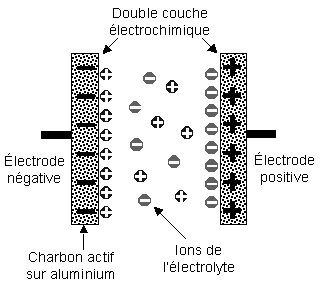
\includegraphics[height=5cm]{supercondensateur.png}
    \caption{Schéma d'un supercondensateur}
    \label{fig:schema_supercondensateur}
\end{figure}

Les électrodes capacitives sont généralement constituées de charbon actif : la porosité de telles électrodes permet d'augmenter la surface de contact avec l'électrolyte pour atteindre des capacitance spécifique de \qtyrange[range-units = single]{100}{300}{\farad \per \gram}.\\
Quant aux électrolytes, ils peuvent être groupés en fonction de leur nature : aqueux, organiques et ioniques. Parmi les électrolytes aqueux se démarquent\cite{zhong_review_2015} les électrolytes acides (\ce{H2SO4}), alkalins (\ce{KOH}), et neutres (\ce{Na2SO4}).

% Presenting the methods and tools
%% Molecular Dynamics and LAMMPS
Lors de cette étude, nous utilisons \emph{Large Atomic/Molecular Massively Parallel Simulator} (LAMMPS) pour effectuer des simulations de Dynamique Moléculaire. En effet, cet outil permet de mettre en place des simulations et d'en contrôler les conditions relativement facilement (contrôle du/des potentiel/s, de l'ensemble thermodynamique, thermostat, barostat, etc.).
%% The data extracting and processing task
Aussi, l'extraction et le traitement des données de simulations ont été une tâche non-négligeable. Pour cela, nous avons utilisé majoritairement des programmes écrits en C dont la conception et réalisation sont détaillées en annexes.\\
%% The additionnal tools
Enfin, pour des outils supplémentaires ont été utilisés pour les tâches restantes comme la visualisation des trajectoires\cite{ovito} ou encore la réalisation de configurations initiales\cite{martinez_packmol_2009}.

% Presenting the plan
La structure des électrodes capacitives étant très complexe du fait du grand nombre de pores et de leur diversité, nous avons préféré adopter un système modèle, que nous présentons en première section.\\
Puis, nous présenterons les outils que nous utilisons pour simuler un supercondensateur en charge, à savoir le potentiel réactif \emph{ReaxFF}\cite{van_duin_reaxff_2001}\cite{russo_atomistic-scale_2011}\cite{senftle_reaxff_2016} et \emph{EChemDID}\cite{onofrio_voltage_2015}.\\
Enfin, nous présentons les résultats obtenus et observations faites lors de cette étude, notamment par rapport à l'adsorption des ions à la surface des électrodes et la répartition des charges en leur sein.

\clearpage

% Presenting the materials and methods
%% Presenting ReaxFF
%%% Theoretical
%%% The LAMMPS implementation
%% Presenting EChemDID
%%% Presenting CC, CV and Qeq
%%% Presenting EChemDID
\section{Présentation des méthodes utilisées}

    Pour cette étude, nous utilisons un certain nombre d'outils et de méthodes que nous présentons dans ci-après, d'autres méthodes et outils, comme le modèle \spce{}, sont présentés brièvement dans les sections où ils sont mentionnés.

Nous effectuons d'abord des rappels de Dynamique Moléculaire car c'est le domaine de notre étude, puis nous présentons \reaxff{} le potentiel réactif que nous utilisons dans nos simulations, et enfin nous discutons d'\echemdid{}, la méthode utilisée pour appliquer la différence de potentiel entre les électrodes.

% Prensenting Molecular Dynamics
    \subsection{Rappels de Dynamique Moléculaire}



% Presenting ReaxFF
    \subsection{Présentation de \reaxff{}} \label{sec:reaxff}

\begin{figure}[h!]
    \centering
    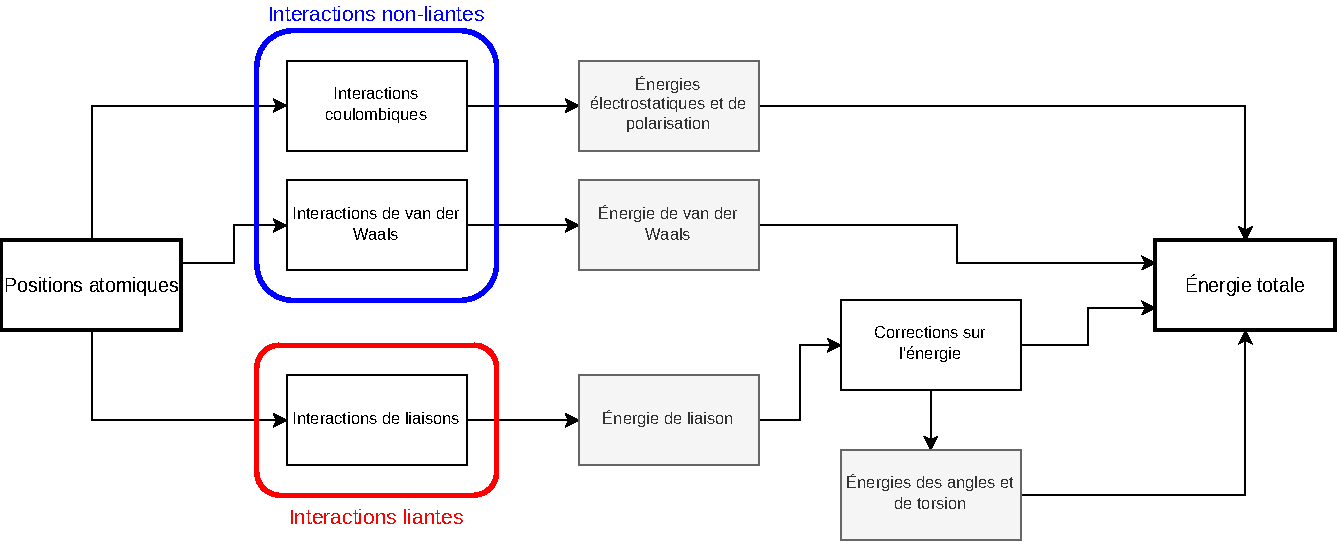
\includegraphics[width=\linewidth]{H2O-ReaxFF-interactions.pdf}
    \caption{Interactions et énergies au sein de \reaxff{} (tiré de \cite{russo_atomistic-scale_2011})}
    \label{fig:interactions_energies_reaxff}
\end{figure}

\reaxff{}\cite{russo_atomistic-scale_2011}\cite{senftle_reaxff_2016} est un potentiel qui utilise les ordres de liaison pour modéliser les réactions chimiques (\autoref{fig:interactions_energies_reaxff}), prend en compte les interaction non-liantes, et effectue  une équilibration de charges.\\
Il a été conçu de façon à obtenir des résultats dont la précision se rapproche des méthodes quantiques, en mettant en jeu autant d'atomes que les méthodes classiques.\\
Enfin, ce potentiel a été comparé à un modèle existant de la molécule d'eau à la \autoref{sec:h2o}.

\textbf{Ordres de liaisons}\\
L'ordre d'une liaison entre un atome $i$ et un atome $j$ est donné par :
\begin{equation}
    BO_{ij}' = \exp \left[p_{bo, 1} \left(\frac{r_{ij}}{r_o}\right)^{p_{bo,2}}\right] + \exp \left[p_{bo,3} \left(\frac{r_{ij}^\pi}{r_o}\right)^{p_{bo,4}}\right] + \exp \left[p_{bo,5} \left(\frac{r_{ij}^{\pi\pi}}{r_o}\right)^{p_{bo,6}}\right]
    \label{eq:ordres_liaisons_reaxff}
\end{equation}
où paramètres $p_{bo,1}, \dots, p_{bo,6}, r_o$ sont des pamramètres issus de calculs \textit{ab initio}, et dépendent de la nature des atomes mis en jeu, et du type de liaison considéré. Les ordres de liaisons sont ensuite corrigés pour être intégrés aux calculs des énergie de liaisons, d'angles et de torsions.

\textbf{Interactions non-liantes}\\
\reaxff{} inclue également les interactions de \vdw{} et \coulomb{} pour \emph{toutes} les paires d'atomes. Les interactions de \vdw{} se basent sur un potentiel de Morse, et ces deux types d'interactions sont écrantées par un paramètre $\gamma$ pour éviter de trop grandes attractions et répulsions (\autoref{fig:reaxff_vdw_coulomb}).

\begin{figure}[h!]
    \centering
    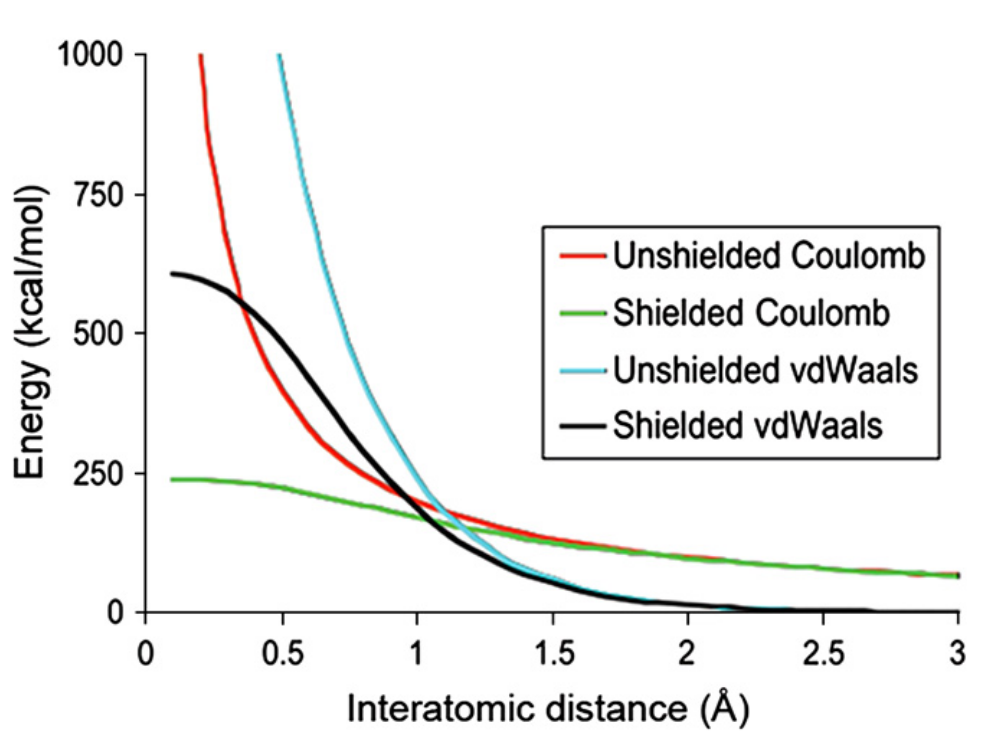
\includegraphics[height = 5 cm]{reaxff_vdw_coulomb.png}
    \caption{Allures des énergies des interactions de \vdw{} et \coulomb{} écrantées {\tiny (tiré de \cite{russo_atomistic-scale_2011})}}
    \label{fig:reaxff_vdw_coulomb}
\end{figure}

\textbf{Équilibration des charges}\\
\reaxff{} utilise une méthode d'équilibration des charges, effectuée à chaque pas de temps, basée sur l'\emph{Electron Equilibration Method} (abrégé \eem{})\cite{mortier_electronegativity-equalization_2002} et la méthode \qeq{}\cite{rappe_charge_1991} :
\begin{equation}
    \boxed%
    {
    \frac{\partial E}{\partial q_i} = \chi_i + 2 q_i H_i + C \sum_{j \neq i} \frac{q_j}{\left(r_{ij}^3 + (1 / \gamma_{ij})^3\right)^{1/3}}
    }
    \ \text{ et } \ 
    \boxed%
    {
        \sum_{i = 1}^{N_{atomes}} q_i = 0
    }
\end{equation}
où $q_i$ est la charge d'un atome $i$, $\chi_i$ son électronégativité, $H_i$ sa dureté, $r_{ij}$ est la distance entre un atome $i$ et un atome $j$ et $\gamma_{ij}$ est le paramètre de protection pour la paire $ij$.


% Presenting EChemDID
    \subsection{Présentation d'\echemdid{}} \label{sec:echemdid}

\begin{figure}[h!]
    \centering
    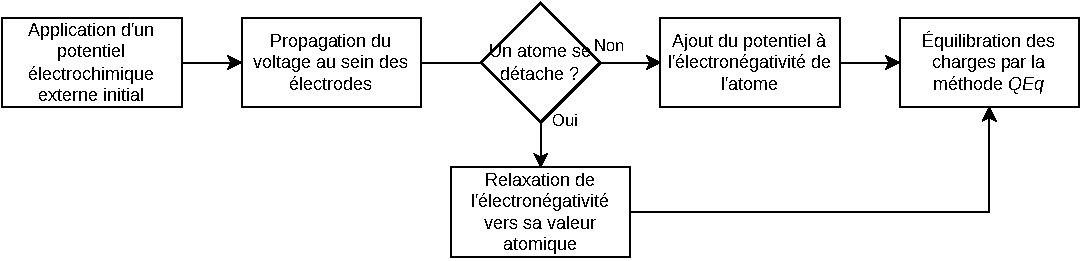
\includegraphics[height = 3 cm]{echemdid_methode.pdf}
    \caption{Fonctionnement d'\echemdid{}}
    \label{fig:echemdid_fonctionnement}
\end{figure}

\textbf{Application d'un potentiel électrochimique externe}\\
Pour fonctionner, \echemdid{} assigne à chaque atome un potentiel électrochimique local $\Phi_i (t)$ et applique initialement un potentiel électrochimique externe à un groupe prédéfini d'atomes.

\textbf{Propagation du voltage au sein des électrodes}\\
Le but d'\echemdid{} étant de représenter les réactions électrochimiques, la progpagation du voltage au sein des électrodes se fait simplement selon la relation :
\begin{equation}
    \dot{\Phi} = k \Delta \Phi
    \label{eq:echemdid_propagation}
\end{equation}
où $k$ est un coefficient de diffusion, et $\Delta$ est l'opérateur Laplacien. Pour résoudre cette équation, \echemdid{} suppose que chaque atome se situe dans un réseau de référence (ou grille).

Pour résoudre cette équation, plusieurs points sont à prendre en compte :
\begin{itemize}
    \item si une différence de potentiel est appliquée entre deux électrodes, le voltage devra s'équilibrer en une durée dépendant du coefficient $k$
    \item si un atome se détache d'une électrode, son électronégativité devra progressivement revenir à sa valeur atomique notée $\chi_i^0$
\end{itemize}

La solution numérique de cette équation peut alors être exprimée :
\begin{equation}
    \boxed%
    {
        \dot{\Phi}_i (t) = \sum_{j \neq i} \frac{\Phi_i (t) - \Phi_j (t)}{{R_{ij}}^2}w(R_{ij}) + \eta F(W_i) \Phi_i
    }
    \label{eq:echemdid_solution_numerique}
\end{equation}
où $R_{ij} = | \vec{r}_i - \vec{r}_j |$, $\vec{r}_i$ est la position de l'atome dans la grille, $w(R)$ est une fonction de poids, $\eta$ est un coefficient de relaxation, $F(W)$ est une fonction d'activation de la relaxation, et $W_i$ est la coordinance métallique totale de l'atome $i$.

Le premier terme à droite de cette équation résout l'équation de la diffusion du voltage aux seins des électrodes, et la fonction de poids a pour expression :
\begin{equation*}
    w(R) = \left\{
        \begin{aligned}
            &\mathcal{N} \left[ 1 - \left(\frac{R}{R_c}\right)^2 \right]^2 &\text{si } R < R_c\\
            &0 &\text{sinon}
        \end{aligned}
    \right.
\end{equation*}
où $R_c$ est la distance maximale à partir de laquelle deux atomes ne sont plus considérés comme faisant partie du même amas métallique, $\mathcal{N} = \frac{2 d N_{atomes}}{\sum_{i} W_i}$ est un coefficient de normalisation, $d$ est le nombre de dimensions du problème, et $W_i = \sum_{j \neq i} w(R_{ij})$ est la coordinance métallique totale de l'atome $i$ sur la grille.

Quant au second terme à droite, il permet d'activer la relaxation de l'électronégativité, et la fonction d'activation a pour expression :
\begin{equation*}
    F(W) = \left\{
        \begin{aligned}
            &\left[ 1 - \left( \frac{W}{W_0}\right)^2\right]^2 &\text{si } W < W_0\\
            &0 &\text{sinon}
        \end{aligned}
    \right.
\end{equation*}
où $W_0$ est la coordinance métallique minimale en dessous de laquelle l'électronégativité doit tendre vers sa valeur atomique, en général on prend $W_0 = w(\num{0.99}R_c)$.

La \autoref{fig:echemdid_allures_w_f} montre l'allure des fonctions $w$ et $F$ pour un réseau cristallin de graphite de \num{540} atomes, en supposant que pour tous les atomes on a $W_i = \num{3}$ et en prenant $R_c = \qty{4}{\angstrom}$.

\begin{figure}[h!]
    \centering
    \begin{subfigure}{\textwidth}
        \centering
        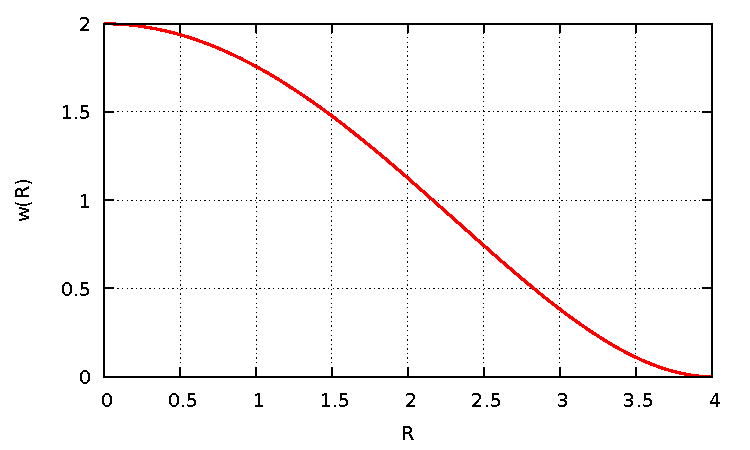
\includegraphics[height = 6 cm]{echemdid_w.pdf}
        \caption{$w(R)$ : {\footnotesize les poids augmentent avec la proximité, ainsi la propagation du voltage est d'autant plus forte que la distance entre deux atomes est petite, et elle s'estompe pour des distances plus grandes que $R_c$.}}
    \end{subfigure}
    \begin{subfigure}{\textwidth}
        \centering
        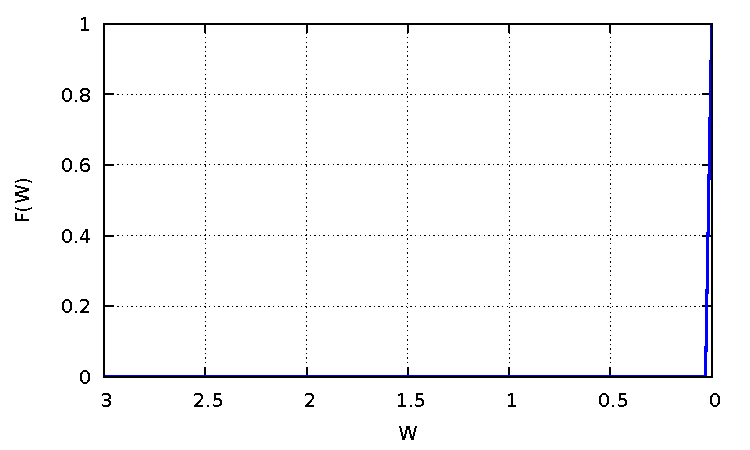
\includegraphics[height = 6 cm]{echemdid_F.pdf}
        \caption{$F(W)$ : {\footnotesize lorsque la coordination métallique diminue, la relaxation s'effectue avec $F$ qui augmente.}}
    \end{subfigure}
    \begin{subfigure}{\textwidth}
        \centering
        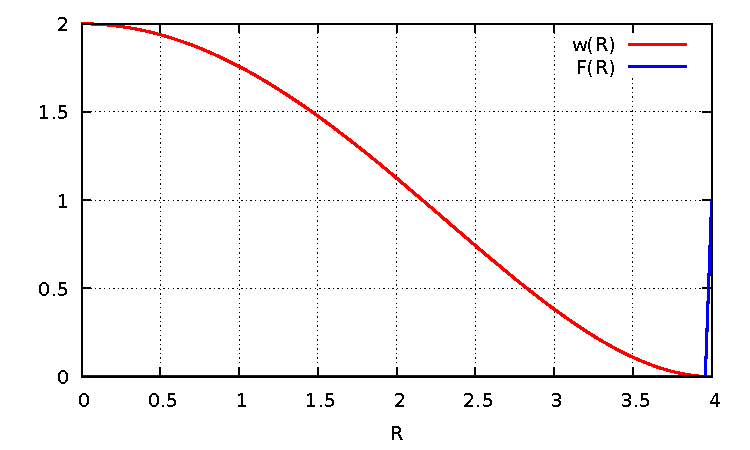
\includegraphics[height = 6 cm]{echemdid_w_F.pdf}
        \caption{$w(R)$ et $F(R) \simeq F(w(R))$ : {\footnotesize les termes ne coexistent quasimment jamais.}}
    \end{subfigure}
    \caption{Allures des fonctions d'\echemdid{}, {\footnotesize pour un réseau cristallin de graphite de \num{540} atomes, en supposant que pour tous les atomes $W = \num{3}$, et en prenant $R_c = \qty{4}{\angstrom}$.}}
    \label{fig:echemdid_allures_w_f}
\end{figure}

\textbf{Ajout du potentiel à l'électronégativité et équilibration des charges}\\
Le potentiel $\Phi_i (t)$ obtenu après avoir calculé la solution (\ref{eq:echemdid_solution_numerique}) et intégré l'\autoref{eq:echemdid_propagation} est ensuite ajouté à l'électronégativité de l'atome $i$ :
\begin{equation*}
    \boxed%
    {
        \chi_i^* (t) = \chi_i^0 + \Phi_i (t)
    }
\end{equation*}
pour effectuer le calcul d'équilibration des charges par la méthode \qeq{}.

\clearpage


% Presenting the model system
%% Interest of the model
%% Description
%% Construction
%% Simulations details
\section{Présentation du système modèle} \label{sec:systeme_modele}

    % Interest of the model
Comme mentionné précédemment, à cause de la complexité du système il est préférable pour cette étude de considérer un sytème modèle. Dans cette section, nous décrivons le modèle et ses caractéristiques, avant de détailler sa construction, et de discuter des simulations dans lesquelles il intervient.

% Description
    \subsection{Description du modèle}

Le système modèle est composé d'électrodes en graphites immergées dans un électrolyte aqueux d'hydroxyde de sodium, sa structure est présentée à la \autoref{fig:schema_structure} et ses caractéristiques au \autoref{tab:caracteristiques_systeme}.

\begin{figure}[h!]
    \centering
    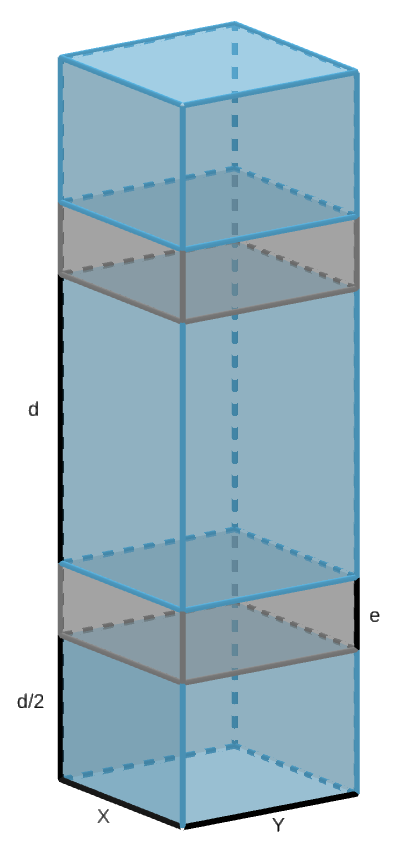
\includegraphics[height = 5 cm]{schema_structure.png}
    \caption{Schéma de la structure du système modèle}
    \label{fig:schema_structure}
\end{figure}

\begin{table}[h!]
    \centering
    \begin{tabular}{l || l | l l}
        \hline
        Groupe &Caractéristique &Valeur &\\
        \hline
        Système &Dimensions &$(22.104, 21.270, \sim 60)$ &\unit{\angstrom}\\
        &Particules &$\sim \num{3000}$ &\\
        \hline
        Électrodes &Séparation &$\sim \num{20}$ &\unit{\angstrom}\\
        &Atomes (par électrode) &\num{540} &\\
        \hline
        Électrolyte &Molécules d'eau &\num{628} &\\
        &Concentration &$\sim \num{1.0}$ &\unit{\mole \per \liter}\\
        &Ions &\num{12} &\\
        \hline
    \end{tabular}
    \caption{Caractéristiques du système}
    \label{tab:caracteristiques_systeme}
\end{table}

% Construction
    \subsection{Construction du modèle}

\begin{figure}[h!]
    \centering
    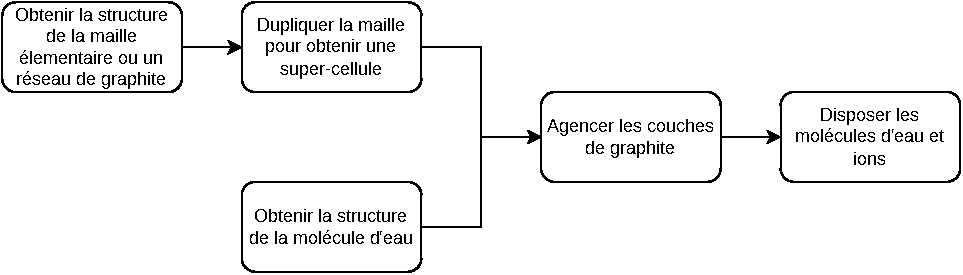
\includegraphics[height = 3 cm]{construction_structure.pdf}
    \caption{Démarche de construction de la structure}
    \label{fig:construction_structure}
\end{figure}

Pour construire la structure du modèle, la démarche \autoref{fig:construction_structure} a été adoptée afin d'obtenir le système aux dimensions et caractéristiques désirées, avec une configuration initiale des particules convenable.

\textbf{Obtention des structures}\\
Les données sur les structures des molécules ont été obtenues grâce à la \href{http://www.crystallography.net/cod/}{Crystallography Open Database} (COD) et celles-ci sont présentées à la \autoref{fig:molecules_initiales}.

\begin{figure}[h!]
	\centering
	\begin{subfigure}[t]{.49\textwidth}
		\centering
		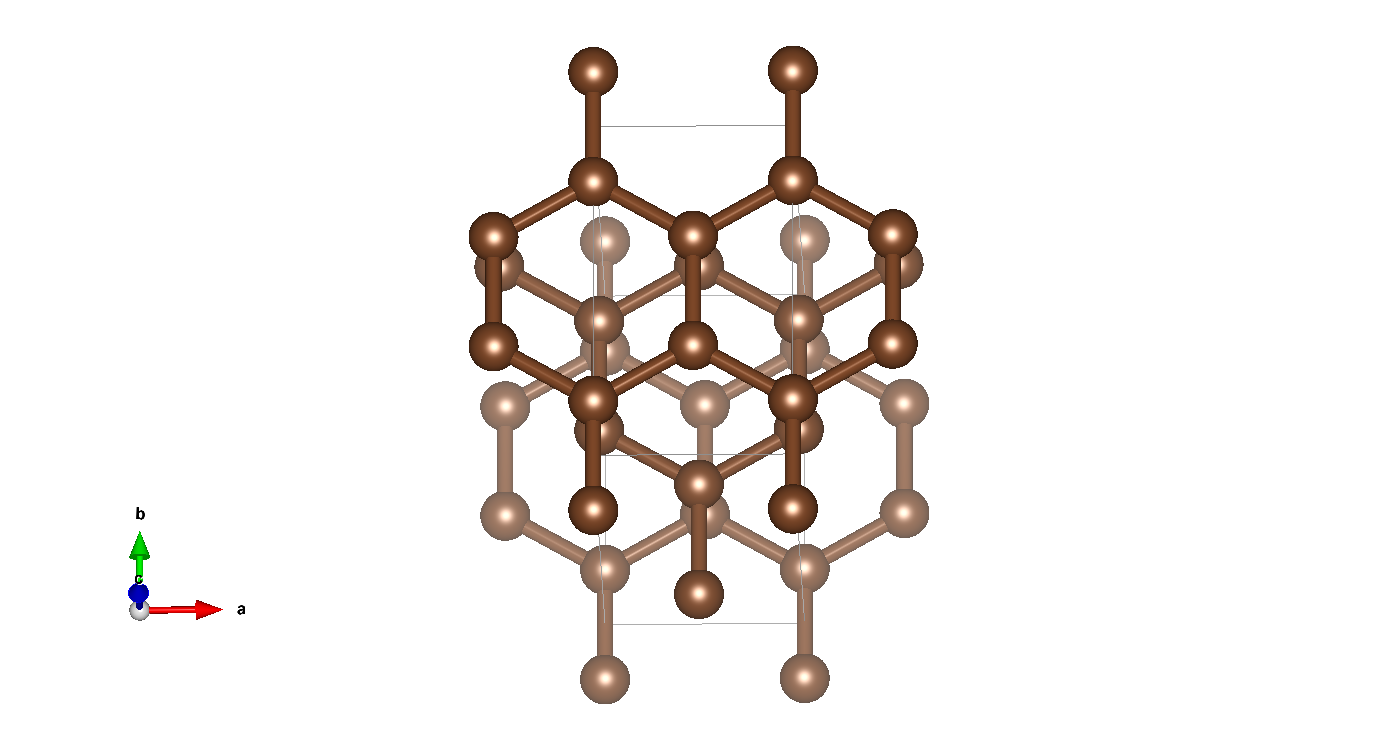
\includegraphics[width = \textwidth]{graphite.png}
		\caption{Réseau de graphite}
	\end{subfigure}%
    ~
	\begin{subfigure}[t]{.49\textwidth}
		\centering
		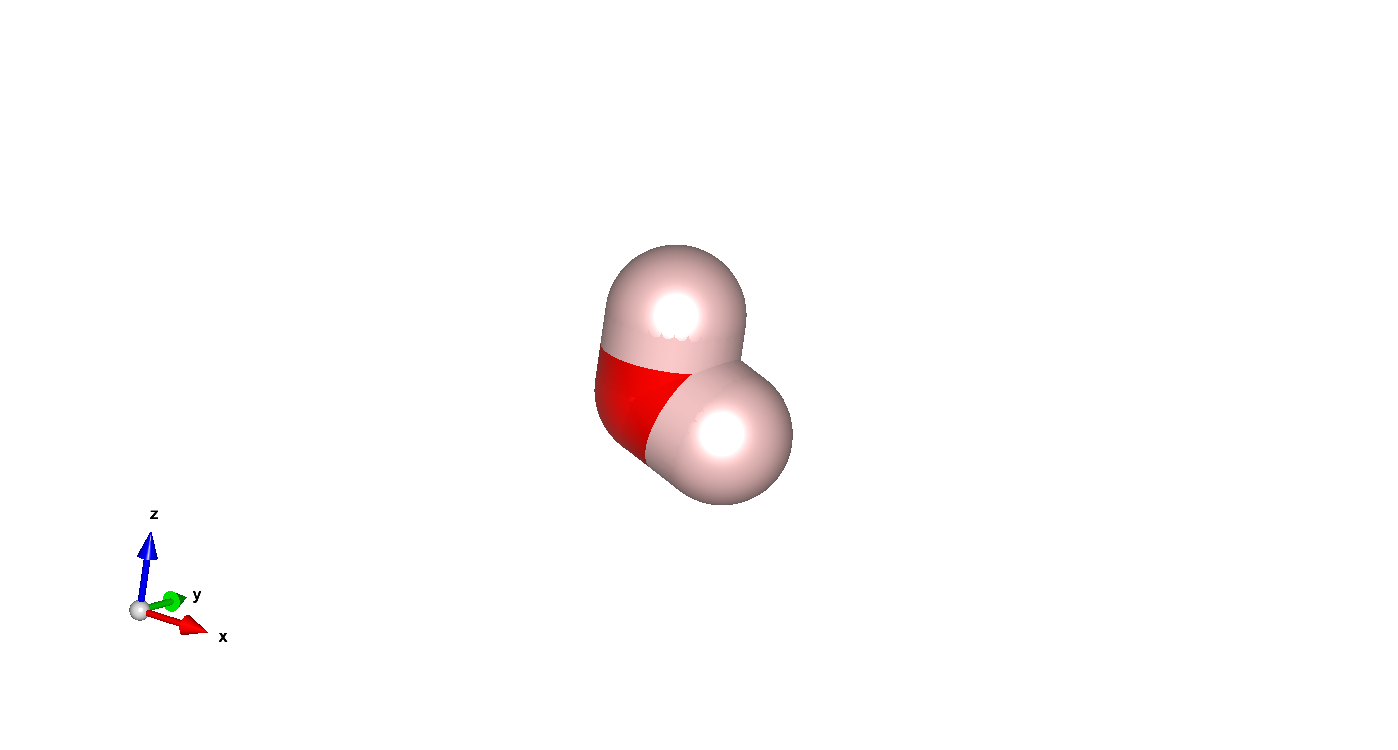
\includegraphics[width = \textwidth]{water.png}
		\caption{Molécule d'eau}
	\end{subfigure}
	\caption{Structures des molécules provenant de la COD}
	\label{fig:molecules_initiales}
\end{figure}

\textbf{Obtention de la super-cellule}\\
La structure de graphite de base a pu être étendue grâce à un logiciel tier\cite{momma_vesta_2011}, \num{9} fois selon la direction $[OX)$ et \num{5} fois selon la direction $[OY)$ afin que les dimensions dans ces directions soient du même ordre, pour obtenir une électrode de graphite (\autoref{tab:dimensions_structures} et \autoref{fig:electrode}).

\begin{table}[h!]
    \centering
    \begin{tabular}{l | c c c}
        \hline
        Structure &X [Å] &Y [Å] &Z [Å]\\
        \hline
        Réseau initial &\num{2.456} &\num{4.254} &\num{6.696}\\
        Électrode de graphite &\num{22.104} &\num{21.270} &\num{6.696}\\
        \hline
    \end{tabular}
    \caption{Dimensions des sctructures}
    \label{tab:dimensions_structures}
\end{table}

\begin{figure}[h!]
    \centering
    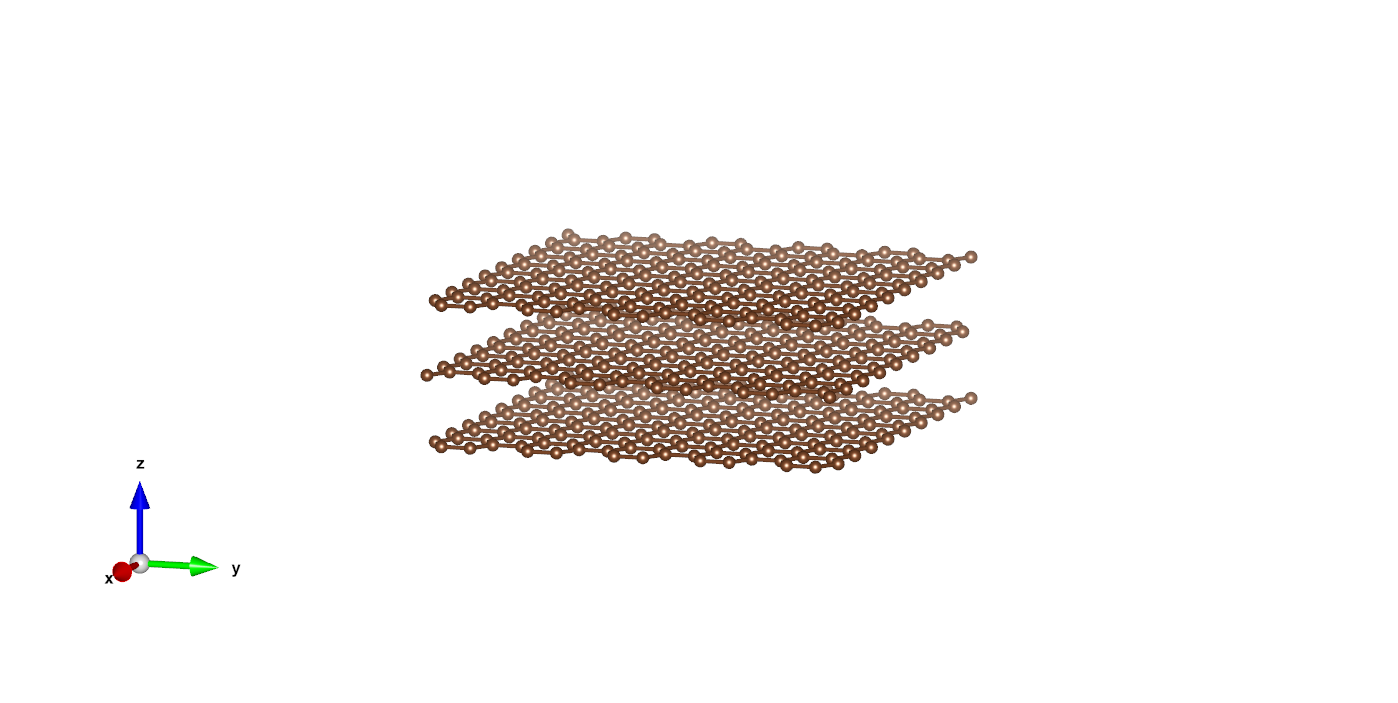
\includegraphics[height = 5 cm]{electrode.png}
    \caption{Électrode obtenue après duplication du réseau de graphite : {\footnotesize les couches de graphènes sont séparées d'environ $\sim$\qty{3.5}{\angstrom}.}}
    \label{fig:electrode}
\end{figure}

\textbf{Agencement des particules}\\
Les particules ont pu être disposées pour construire le modèle à l'aide de \packmol{}\cite{martinez_packmol_2009}, détails à l'\autoref{apdx:packmol}.

Pour obtenir des configurations initiales suffisamment stables nous avons choisi de répartir les entités en les séparant d'au moins \qty{2.5}{\angstrom} : entre les molécules et ions de l'électrolyte, et entre les particules de l'électrolyte et les électrodes.\\
Et pour respecter les conditions aux limites périodiques, cette séparation a également été appliquée aux bords du système : nous ajoutons un retrait égal à la moitité de cette séparation à chaque bord.

Finalement, nous obtenons la configuration présentée à la figure \autoref{fig:structure_finale}.

\begin{figure}[h!]
    \centering
    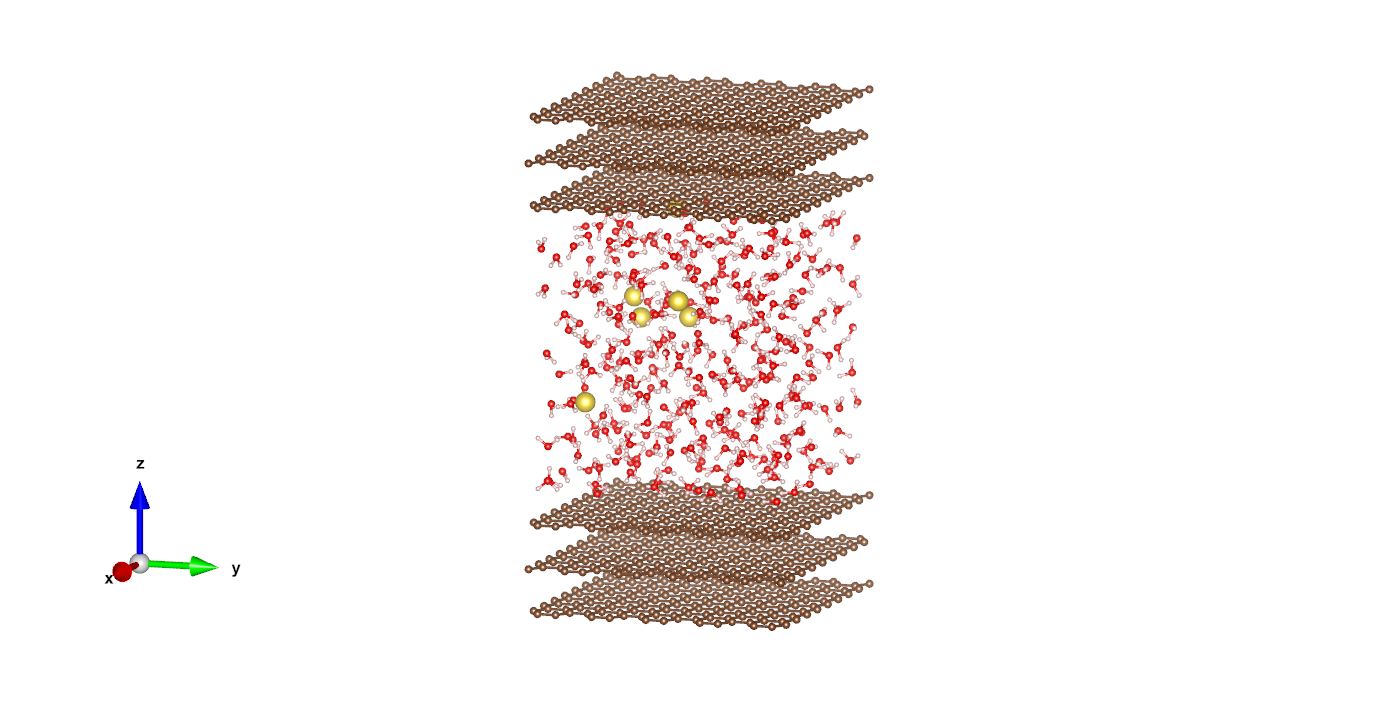
\includegraphics[height = 5 cm]{structure.png}
    \caption{Structure finale obtenue après agencement des molécules}
    \label{fig:structure_finale}
\end{figure}

% Simulations details
    \subsection{Déroulement et détails des simulations} \label{sec:deroulement_simulations}

\begin{table}[h!]
    \centering
    \begin{tabular}{l || l | l l}
        \hline
        Étape &Paramètre &Valeur &\\
        \hline
        Toutes &\lstinline!timestep! &\num{0.1} &\unit{\femto \second}\\
        &potentiel &\reaxff{} &\\
        \hline
        Minimisation &\lstinline!maxiter! &\num{1000} &\\
        &\lstinline!maxeval! &\num{10000} &\\
        &\lstinline!etol! &\num{e-05} &\\
        &\lstinline!ftol! &\num{e-06} &\unit{\kilo \cal \per \mole \per \angstrom}\\
        \hline
        Relaxation et Stabilisation &durée &\num{200000} &\\
        & &\num{20.0} &\unit{\pico \second}\\
        &\lstinline!T_target! &\num{300.0} &\unit{\kelvin}\\
        &\lstinline!P_target! &\num{1.0} &\unit{\atm}\\
        \hline
        Simulation &durée &\num{10000000}\\
        &polarisation &\echemdid{} &\\
        & &\num{1.0} &\unit{\nano \second}\\
        &\lstinline!T_target! &\num{300.0} &\unit{\kelvin}\\
        \hline
    \end{tabular}
    \caption{Récapitulatif des paramètres des simulations}
\end{table}

\begin{figure}[h!]
    \centering
    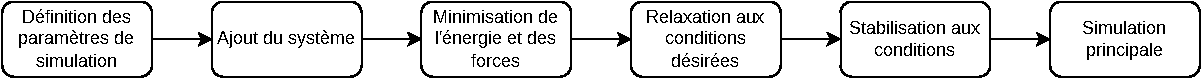
\includegraphics[width = \textwidth]{deroulement_simulations.pdf}
    \caption{Déroulement des simulations}
    \label{fig:deroulement_simulations}
\end{figure}

Toutes les simulations suivent le déroulement de la \autoref{fig:deroulement_simulations} afin de définir les paramètres de simulation, de préparer le système, et de lui permettre de s'équilibrer.

\textbf{Paramétrisation}\\
Elle consiste à définir les paramètres clés de la simulation. Par exemple :
\begin{itemize}
    \item le pas de temps (\lstinline!timestep!) sélectionné pour les simulations est de \qty{0.1}{\femto \second}
    \item les interactions sont basés sur le potentiel réactif \reaxff{} (détaillé à la \autoref{sec:reaxff})
    \item la mise en place de la différence de potentiel entre les électrodes est réalisée grâce à \echemdid{} (détaillé à la \autoref{sec:echemdid})
\end{itemize}

\textbf{Ajout du système}\\
Ceci est effectué avec une commande \lammps{} de lecture de données. Pour ce faire, il est nécessaire de convertir les données des positions des particules du système (détails à la \autoref{sec:systeme_modele}) en données \lammps{} (détails à l'\autoref{apdx:conversion_lammps}).

\textbf{Minimisation}\\
Cette étape est essentielle au démarrage d'une simulation : elle sert à s'assurer que la configuration de départ de la simulation soit "correcte" et que le système soit stable.

Elle consiste à déplacer les particules du système sans dynamique de manière à minimiser l'énergie potentielle et les forces totales du système. Cette procédure suit un algorithme de gradient conjugué avec pour fonction objectif l'énergie potentielle totale :
\begin{equation*}
    E(r_1, \dots, r_N) = \sum_{i, j} E_{pair} (r_i, r_j) + \dots + \sum_{i, j} E_{fix} (r_i)
\end{equation*}
où sont prises en compte les énergies :
\begin{itemize}
    \item des interactions de paires
    \item des liaisons et angles si présents
    \item des interactions \textit{improper} ou \textit{dihedral} : les interactions mettant en jeu \num{3} ou \num{4} atomes
    \item des \lstinline!fix! imposés lors de la minimisation : des commandes \lammps{} visant à imposer des contraintes lors de la minimisation, par exemple la relaxation de la boîte pour atteindre une pression désirée, ou encore les forces désactivées pour un groupe d'atomes pour qu'ils ne subissent pas de modifications
\end{itemize}

\textbf{Relaxation et stabilisation}\\
Ces étapes utilisent un thermostat et barostat de Nosé--Hoover pour atteindre les conditions physiques recherchées et les stabiliser.

Les conditions de pression et de température recherchées sont $T = \qty{300}{\kelvin}$ et $P = \qty{1}{\atm}$, et les évolutions des quantités thermodynamiques lors de ces étapes sont typiquement celles des \autoref{fig:allures_thermostat_barostat}.

\begin{figure}[h]
    \centering
    \begin{subfigure}[t]{.49\textwidth}
        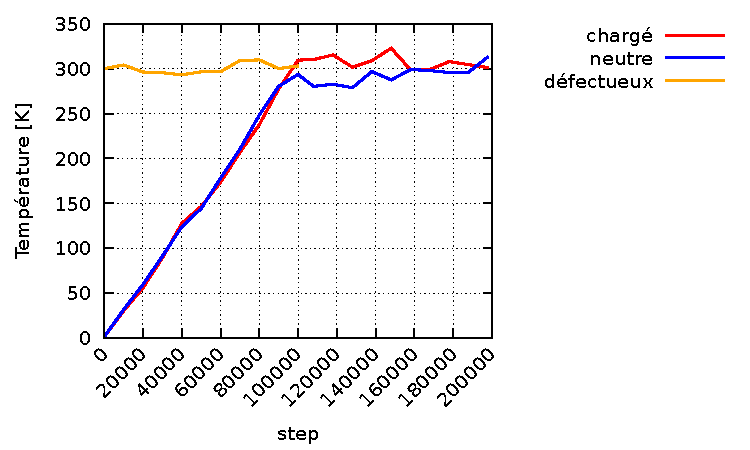
\includegraphics[width = \textwidth, draft]{relaxation_temp.pdf}
        \caption{Température}
    \end{subfigure}%
    ~
    \begin{subfigure}[t]{.49\textwidth}
        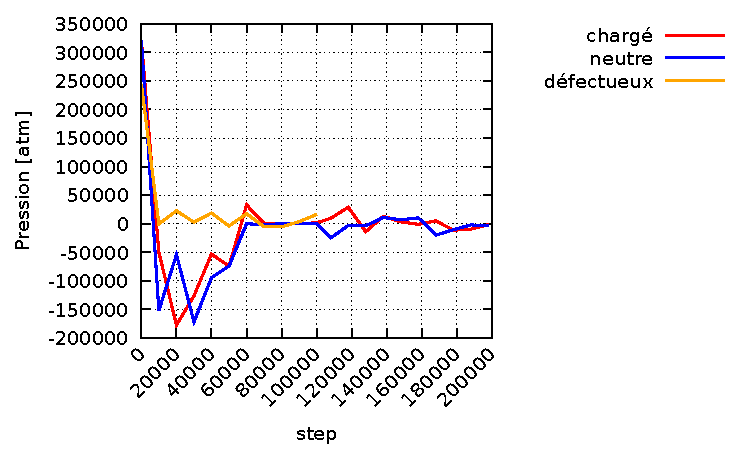
\includegraphics[width = \textwidth, draft]{relaxation_press.pdf}
        \caption{Pression}
    \end{subfigure}
    \begin{subfigure}[t]{.49\textwidth}
        \includegraphics[width = \textwidth, draft]{relaxation_density.pdf}
        \caption{Densité}
    \end{subfigure}
    \caption{Allures des grandeurs thermodynamiques pendant de la relaxation et la stabilisation {\tiny (chaque étape a lieu en \num{100000} \lstinline!timestep!s soit \qty{10}{\pico \second})}}
    \label{fig:allures_thermostat_barostat}
\end{figure}

\textbf{Simulation}\\
Cette étape sert à récolter des données et informations sur le système après qu'il a atteint l'équilibre.

Elle se déroule avec un thermostat de Nosé--Hoover à \qty{300}{\kelvin} et pour une durée $\geq~\qty{1}{\nano \second}$ (\autoref{fig:allures_simulation_principale}).

\begin{figure}[h]
    \centering
    \begin{subfigure}[t]{.49\textwidth}
        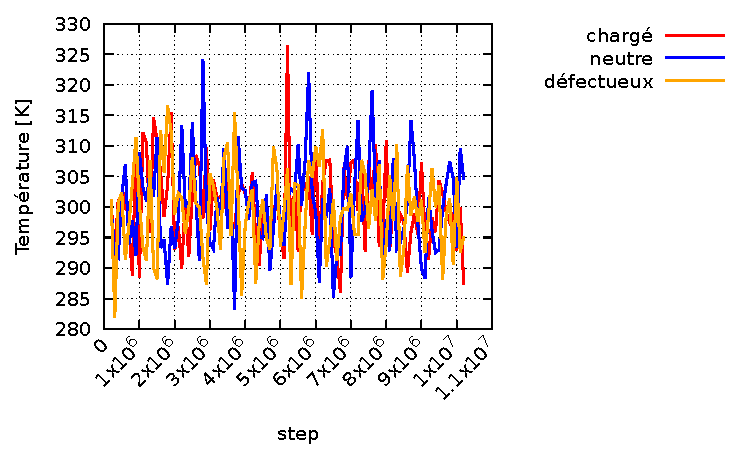
\includegraphics[width = \textwidth, draft]{main_temp.pdf}
        \caption{Température}
    \end{subfigure}%
    ~
    \begin{subfigure}[t]{.49\textwidth}
        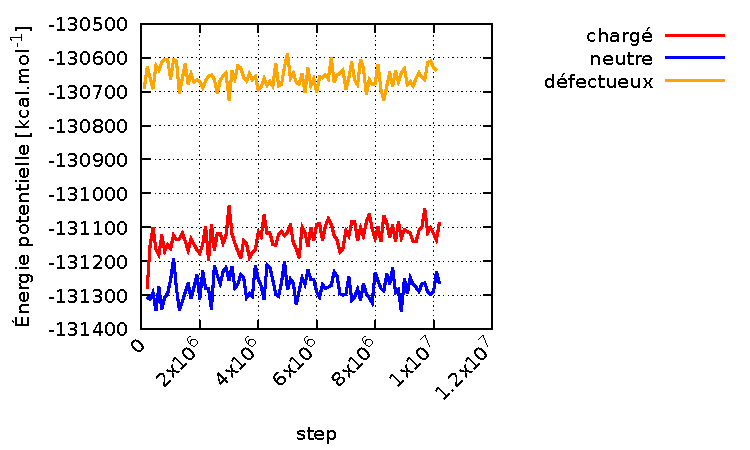
\includegraphics[width = \textwidth, draft]{main_epot.pdf}
        \caption{Énergie potentielle}
    \end{subfigure}
    \begin{subfigure}[t]{.49\textwidth}
        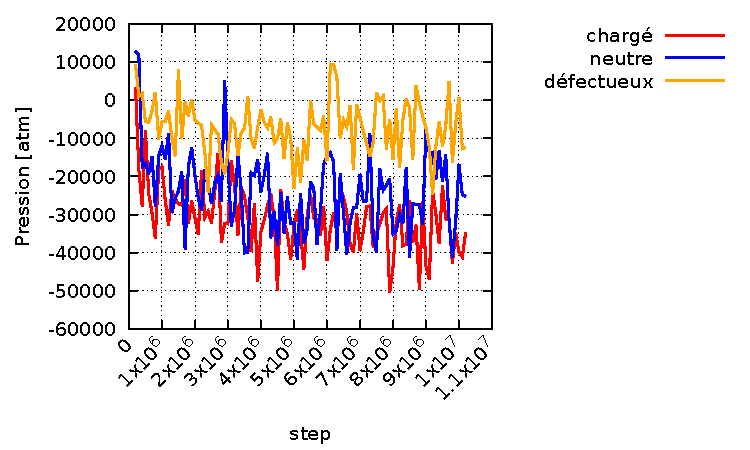
\includegraphics[width = \textwidth, draft]{main_press.pdf}
        \caption{Pression}
    \end{subfigure}
    \caption{Allures des grandeurs thermodynamiques pendant la simulation principale}
    \label{fig:allures_simulation_principale}
\end{figure}

\clearpage


% Presenting the results
%% Comparing two methods for the modeling of water
%% Charge distribution
%% Ions adsorption/displacement
\section{Résultats et discussion}

    % Comparing two methods for the modeling of water
\subsection{Comparaison de deux méthodes pour modéliser la molécule d'eau} \label{sec:h2o}

Puisque l'eau joue un rôle important dans le système que nous étudions, nous voulons explorer plusieurs approches pour la modélisation de la molécule d'eau :
\begin{itemize}
    \item le modèle \emph{Extended Simple Point Charge} (abrégé \spce{})\cite{pullman_interaction_1981}\cite{berendsen_missing_1987}
    \item le potentiel réactif \reaxff{} (présenté à la \autoref{sec:reaxff})
\end{itemize}

C'est également un système suffisamment simple pour une prise en main de \lammps{} et de simulations de Dynamique Moléculaire.

Nous faisons d'abord une brève comparaison des fonctionnements théoriques des deux méthodes, puis mettons en place des simulations d'un même système avec ces deux approches, et finalement comparons leurs résultats.

\textbf{Comparaison des fonctionnements}\\
Alors que le potentiel \reaxff{} est réactif et se base sur les ordres de liaison (voir \autoref{sec:reaxff}), le modèle \spce{} est rigide et les interactions intermoléculaires ne considèrent que les atomes d'oxygène avec un potentiel de Lennard--Jones (\autoref{fig:spce_lj} et \autoref{tab:comparaison_modeles}).

\begin{figure}[h!]
    \centering
    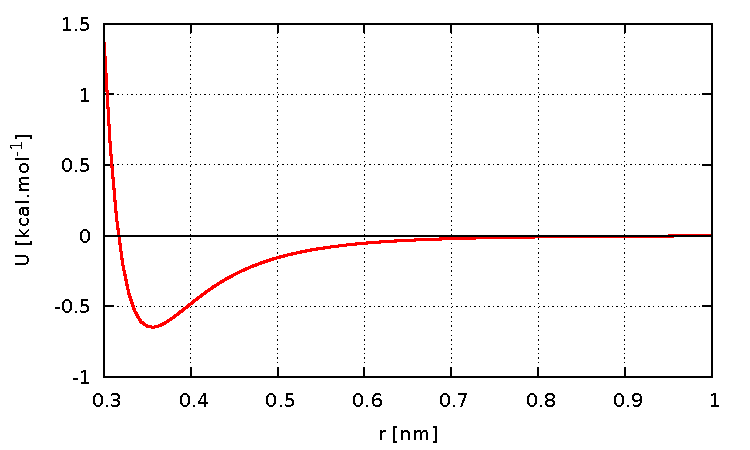
\includegraphics[height = 5 cm]{spce_lj.pdf}
    \caption{Potentiel de Lennard--Jones du modèle \spce{} : {\footnotesize les paramètres de Lennard--Jones sont $A = \qty{0.37122}{(\kilo \cal \per \mol)\tothe{1/6} \nano \meter}$ et $B = \qty{0.3428}{(\kilo \cal \per \mol)\tothe{1/12} \nano \meter}$}}
    \label{fig:spce_lj}
\end{figure}

\begin{table}[h!]
    \centering
    \begin{tabular}{l || c | c}
        \hline
        Caractéristiques               & \reaxff{}         & \spce{}           \\
        \hline
        Modèle de liaisons             & Ordres de liaison & Rigide/Harmonique \\
        Modèle d'angles                & Ordres de liaison & Rigide/Harmonique \\
        Modèle de molécules            & Aucun             & Rigide            \\
        Interactions intermoléculaires & \reaxff{}         & Lennard--Jones    \\
        \hline
    \end{tabular}
    \caption{Comparaison des fonctionnements des modèles}
    \label{tab:comparaison_modeles}
\end{table}

De fait, \reaxff{} est un potentiel objectivement plus flexible que le modèle \spce{} mais implique une charge de calcul beaucoup plus grande.

Par ailleurs, puisque le modèle \spce{} fait appel à des molécules/liaisons/angles rigides, son utilisation avec \lammps{} nécessite l'utilisation d'un format de données de configuration initiale plus complet que \reaxff{}. La conversion des données dans ce format est détaillée à l'\autoref{apdx:conversion_spce}.

\textbf{Mise en place des simulations}\\
Pour faciliter la comparaison des résultats obtenus par simulations aux résultats expérimentaux, les conditions de simulations sont : $T = \qty{300}{\kelvin}, P = \qty{1}{\atm}$.\\
De plus, les simulations suivent un déroulement similaire à celui présenté à la \autoref{sec:deroulement_simulations}, c'est-à-dire :
\begin{itemize}
    \item Une minimisation à \qty{0}{\kelvin}
    \item Une relaxation de \qtyrange{1}{300}{\kelvin} et à \qty{1}{\atm} en \qty{10}{\pico \second}
    \item Une stabilisation de \qty{10}{\pico \second}
    \item La simulation principale pour \qty{1}{\nano \second}
\end{itemize}
et mettent en jeu \num{267} molécules d'eau initialement dans une boîte cubique de côté \qty{20}{\angstrom}.

Les différentes quantités thermodynamiques relevées au cours de ces simulations sont présentées aux \autoref{fig:h2o_relaxation} et \ref{fig:h2o_main}.

\begin{figure}[h!]
    \centering
    \begin{subfigure}{.49\textwidth}
        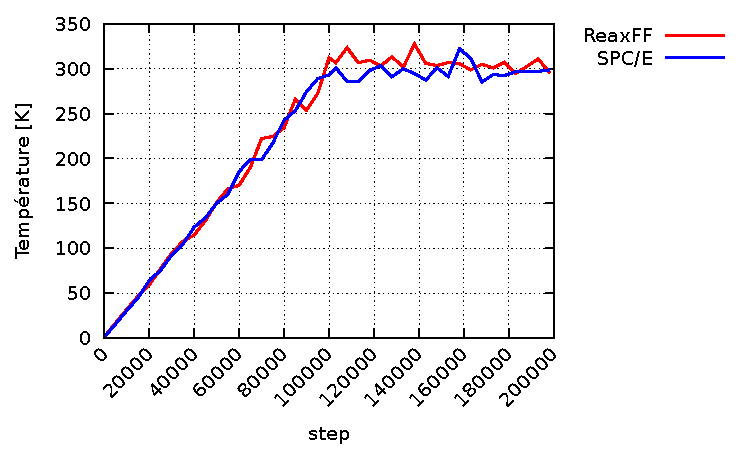
\includegraphics[width = \textwidth]{h2o_relaxation_temp.pdf}
        \caption{Températures}
    \end{subfigure}%
    ~
    \begin{subfigure}{.49\textwidth}
        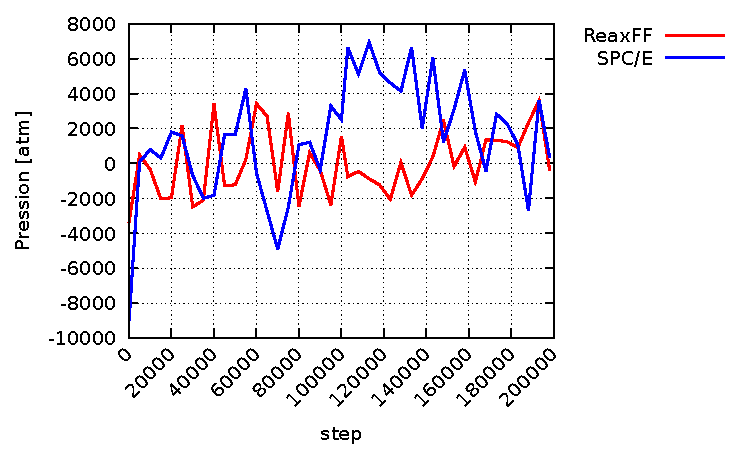
\includegraphics[width = \textwidth]{h2o_relaxation_press.pdf}
        \caption{Pressions}
    \end{subfigure}
    \begin{subfigure}{.49\textwidth}
        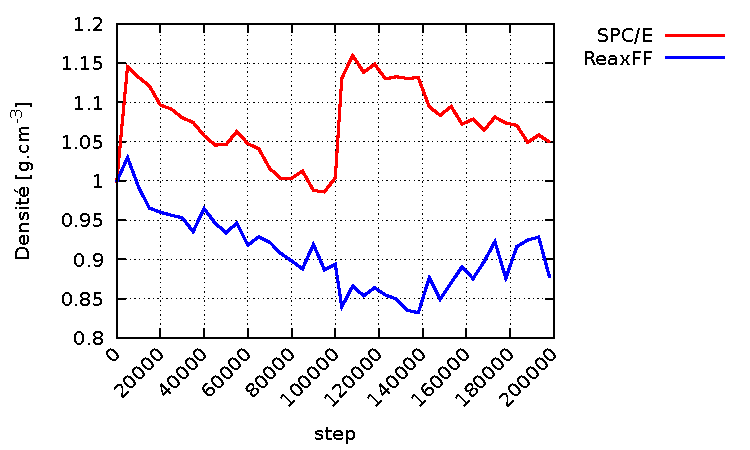
\includegraphics[width = \textwidth]{h2o_relaxation_density.pdf}
        \caption{Densités}
    \end{subfigure}
    \caption{Quantités thermodyanmiques lors de la relaxation}
    \label{fig:h2o_relaxation}
\end{figure}

\begin{figure}[h!]
    \centering
    \begin{subfigure}{.49\textwidth}
        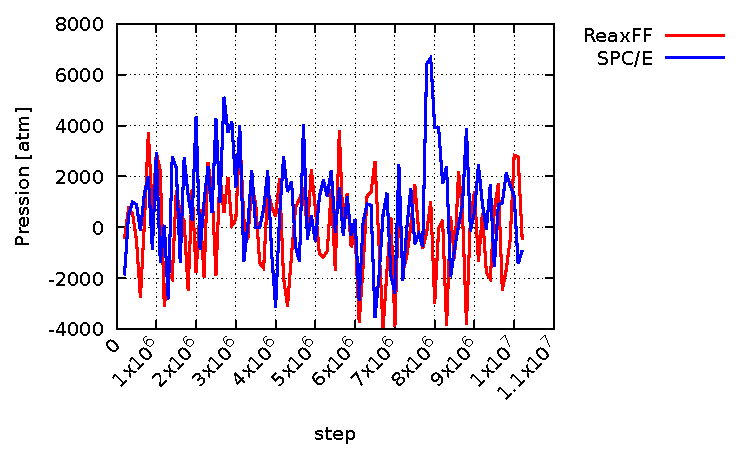
\includegraphics[width = \textwidth]{h2o_main_press.pdf}
        \caption{Pressions}
    \end{subfigure}%
    ~
    \begin{subfigure}{.49\textwidth}
        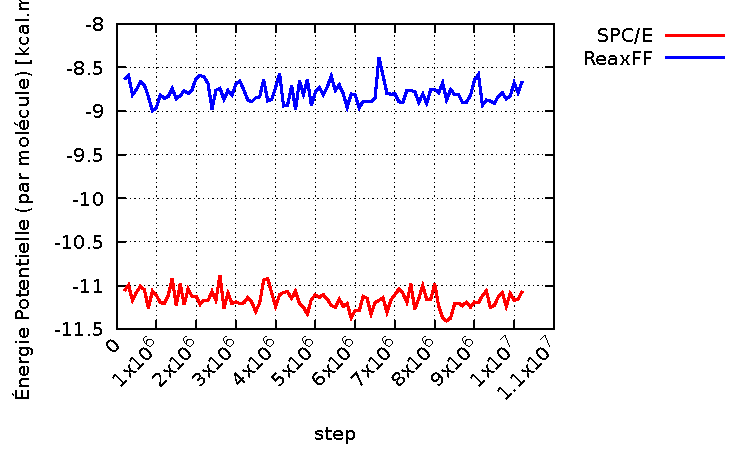
\includegraphics[width = \textwidth]{h2o_main_epot.pdf}
        \caption{Énergies potentielles totales}
    \end{subfigure}
    \caption{Quantités thermodynamiques lors de la simulation}
    \label{fig:h2o_main}
\end{figure}

\textbf{Proriétés comparées}\\
Pour cette étude, nous comparons les propriétés structurales et de diffusion des deux modèles avec la \emph{Radial Distribution Function} et le \emph{Mean Squared Displacement}.

En effet, pour rappel, la première des deux grandeurs nous informe sur la probabilité de trouver deux atomes à une distance donnée l'un de l'autre en comparaison à un gaz parfait :
\begin{equation}
    \boxed%
    {
        g (r) = \frac{\left\langle \rho (r) \right\rangle}{\rho} = \frac{\mathrm{d}n(r)}{4 \pi r^2 \mathrm{d}r \rho}
    }
    \label{eq:rdf}
\end{equation}
où $\rho (r)$ est la densité locale de particules, $\left\langle \cdot \right\rangle$ est la moyenne sur l'ensemble, $\mathrm{d}n(r)$ est le nombre de particules à l'intérieur de la coquille sphérique située à $r$ et d'épaisseur $\mathrm{d}r$, et $\rho$ est la densité numérique moyenne de la paire considérée.

Quant à la deuxième quantité, pour des temps sufisamment longs elle nous donne indirectement le coefficient de diffusion du système :
\begin{equation*}
    MSD(t) \equiv \left\langle \left| \vec{r}(t) - \vec{r}(t_0) \right|^2 \right\rangle = 2 d D t
\end{equation*}
où $\vec{r}$ est la position d'une particule, $\left\langle \cdot \right\rangle$ est la moyenne sur l'ensemble, $t_0$ est un temps de référence, $d$ est le nombre de dimensions du problème, $D$ est le coefficient de diffusion du système et $t$ est le temps.

Cependant, pour obtenir une meilleur précision quant au coefficient de diffusion, nous utilisons le \emph{Mean Squared Displacement} moyenné sur les décalages en temps :
\begin{equation}
    \boxed%
    {
        \overline{MSD} (\tau) = \frac{1}{N_{\tau}} \sum_{i = 0}^{N_{\tau}} \left\langle \left| \vec{r}(\tau) - \vec{r}(t_0) \right|^2 \right\rangle  = 2 d D t
    }
\end{equation}
où $\tau$ est un décalage de configurations, et $N_{\tau}$ le nombre de configurations pouvant être décalées de $\tau$ dans la trajectoire. $\overline{MSD}$ est donc, pour chaque décalage de configurations, une moyenne sur l'ensemble de la trajectoire.

\textbf{Résultats obtenus}\\
Nous présentons et discutons des résultats obtenus ci-dessous. Il est important de préciser qu'\textit{a priori} nous attendons des deux modèles une bonne correspondance avec les résultats expérimentaux, c'est-à-dire moins de \qty{15}{\percent} d'erreurs relatives ; Et cela car d'un côté \spce{} est un modèle exclusivement conçu pour la molécule d'eau et de l'autre \reaxff{} se base sur des résultats très précis issus de simulations \textit{ab initio}.

Les résultats obtenus à l'issue des simulations sont comparées aux valeurs expérimentales correspondantes\cite{soper_radial_2000}\cite{tsimpanogiannis_self-diffusion_2019} (\autoref{tab:h2o_rdf} et \ref{tab:h2o_diffusion}).

\begin{table}[h!]
    \centering
    \begin{tabular}{l | c c | c c}
        \hline
        Données &1\textsuperscript{er} max. [\unit{\angstrom}] &$g$\textsubscript{\ce{OH}} &2\textsuperscript{e} max. [\unit{\angstrom}] &$g$\textsubscript{\ce{OH}}\\
        \hline
        Expérimentale\cite{soper_radial_2000} &\num{0.93} &\num{11.66} &\num{1.80} &\num{1.15}\\
        \reaxff{} &\num{0.94} &\num{22.18} &\num{1.84} &\num{1.35}\\
        \spce{} &\num{1.00} &\num{23.99} &\num{1.72} &\num{1.71}\\
        \hline
    \end{tabular}
    \begin{tabular}{c c | c c}
        \hline
        1\textsuperscript{er} max. [\unit{\angstrom}] &$g$\textsubscript{\ce{OO}} &2\textsuperscript{e} max. [\unit{\angstrom}] &$g$\textsubscript{\ce{OO}}\\
        \hline
        \num{2.74} &\num{2.94} &\num{4.45} &\num{1.18}\\
        \num{2.83} &\num{2.78} &\num{4.45} &\num{1.20}\\
        \num{2.76} &\num{3.14} &\num{4.44} &\num{1.16}\\
        \hline
    \end{tabular}
    \caption{Résultats pour les \emph{Radial Distribution Function}s}
    \label{tab:h2o_rdf}
\end{table}

\begin{table}[h!]
    \centering
    \begin{tabular}{l || c | c}
        \hline
        Données &Coefficient de diffusion (\unit{\square \meter \per \second}) &Erreur relative (\unit{\percent})\\
        \hline
        Expérimentale\cite{tsimpanogiannis_self-diffusion_2019} &\num{2.30e-9} &--\\
        \reaxff{} &\num{2.45e-9} &\num{6.5}\\
        \spce{} &\num{1.61e-9} &\num{30}\\
        \hline
    \end{tabular}
    \caption{Résultats pour les coefficients de diffusion}
    \label{tab:h2o_diffusion}
\end{table}

Pour les \emph{Radial Distribution Function}s, nous comparons les pics que nous jugeons les plus importants, c'est-à-dire :
\begin{itemize}
    \item l'abscisse du premier maximum de $g_{\ce{OH}}$ donnant des indications sur la longueur de la liaison \ce{OH} ; L'intensité des pics n'est pas prise en compte car elle trop sensible à la valeur de la largeur $\mathrm{d}r$ et à la précision du calcul de la $g_{\ce{OH}}$
    \item le second maximum de la $g_{\ce{OH}}$, caractéristique des liaisons hydrogène de la molécule d'eau
    \item le premier maximum de la $g_{\ce{OO}}$, indicateur des distances intermoléculaires (notamment pour \spce{})
    \item le second maximum de la $g_{\ce{OO}}$
\end{itemize}

\reaxff{} a de meilleurs résultats que le modèle \spce{} pour l'abscisse du premier pic de la $g_{\ce{OH}}$ [\qty{1.1}{\percent} contre \qty{7.5}{\percent}], pour le second pic de la $g_{\ce{OH}}$ [\qty{2.2}{\percent} contre \qty{4.4}{\percent} en absicce ; \qty{17.4}{\percent} contre \qty{48.7}{\percent} en intensité], pour l'intensité du premier pic de la $g_{\ce{OO}}$ [\qty{5.4}{\percent} contre \qty{6.8}{\percent}], et pour l'abscisse du second pic de la $g_{\ce{OO}}$ où il correspond exactement à la valeur expérimentale.

De l'autre côté, le modèle \spce{} a de meilleurs résultats que \reaxff{} pour l'abscisse du premier pic de la $g_{\ce{OO}}$ [\qty{0.7}{\percent} contre \qty{3.3}{\percent}].

Enfin, les modèles ont la même erreur pour l'intensité du second pic de la $g_{\ce{OO}}$ [\qty{1.7}{\percent}].

\begin{figure}[h!]
    \centering
    \begin{subfigure}{\textwidth}
        \centering
        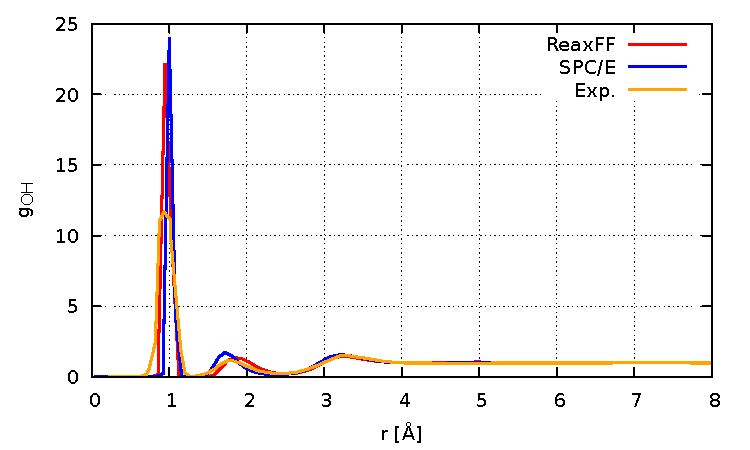
\includegraphics[width = \textwidth]{h2o_rdf_oh.pdf}
        \caption{Pour la paire \ce{OH} : \reaxff{} a de meilleurs résultats que \spce{} sur tous les points, cependant les deux modèles présentent de grandes erreurs pour l'intensité du second pic}
        \label{fig:h2o_rdf_oh}
    \end{subfigure}

    \begin{subfigure}{\textwidth}
        \centering
        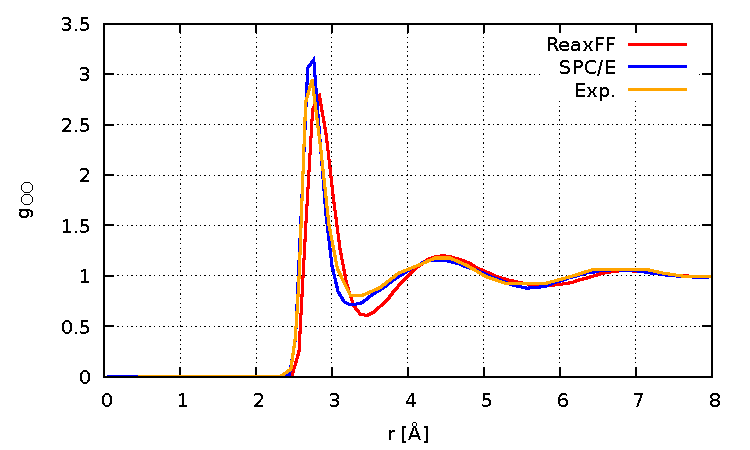
\includegraphics[width = \textwidth]{h2o_rdf_oo.pdf}
        \caption{Pour la paire \ce{OO} : \spce{} représente mieux l'abscisse du premier pic mais \reaxff{} a une erreur moindre quant à son intensité ; Les deux modèles ont de bons résultats pour le second pic}
        \label{fig:h2o_rdf_oo}
    \end{subfigure}
    \caption{Comparaison des \emph{Radial Distribution Function}s : même si les erreurs relatives restent globalement correctes, \reaxff{} a plus souvent de meilleurs résultats par rapport aux points comparés}
    \label{fig:h2o_comparaison_resultats}
\end{figure}

\begin{figure}[h!]
    \centering
    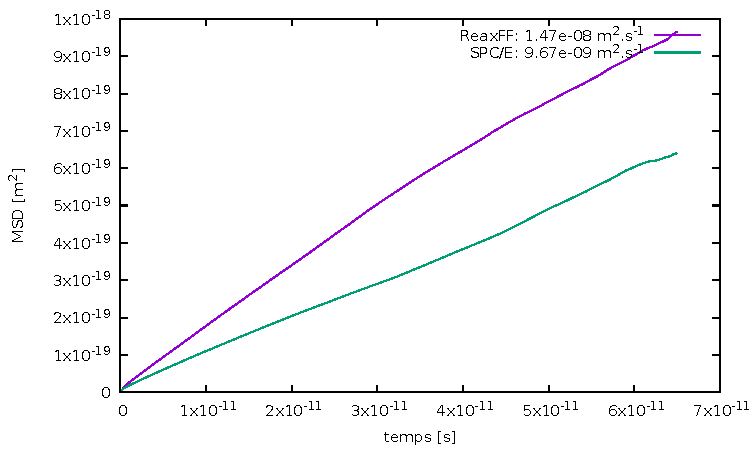
\includegraphics[width = \textwidth]{h2o_msd.pdf}
    \caption{Comparaison des \emph{Mean Squared Displacement}s : les coefficients de diffusion sont calculés avec les pentes de ces courbes ; Pour les deux courbes on a $R = 0.99$}
    \label{fig:h2o_msd}
\end{figure}

Pour les \emph{Mean Squared Displacement}s, \reaxff{} modélise mieux la diffusion que le modèle \spce{} [\qty{6.5}{\percent} contre \qty{30}{\percent}]. Nous pouvons supposer que cette grande différence est due au fait que le modèle \spce{} n'a pas été pensé pour représenter la diffusion de la molécule mais sa polarité.

\clearpage
    % Supercapacitor results
    \subsection{Comportement du système}

Les comportements du système ont ensuite été étudiés. Comme nous l'avons évoqué précédemment, nous souhaitons étudier la distribution des charges au sein des électrodes et les phénomènes d'adsorption des ions.

Pour ce faire, nous avons imaginé trois systèmes : un système chargé à \qty{4.0}{\volt}, un système non chargé, et un système chargé à \qty{4.0}{\volt} comportant un défaut sur une des électrodes. Le défaut choisi a été un atome de carbone manquant.\\
Pour chacun d'eux, deux simulations ont été effectuées : pour un nombre arbitraire d'ions (\num{10} paires d'ions entre les électrodes), et pour une concentration d'\qty{1}{\mole \per \liter} (soit \num{2} paires d'ions entre les électrodes).

Chacune de ces simulations a suivi le déroulement de la \autoref{sec:deroulement_simulations}, c'est-à-dire :
\begin{itemize}
    \item une minimisation à \qty{0}{\kelvin}
    \item une relaxation à \qty{300}{\kelvin} et \qty{1}{\atm} en deux étapes de \qty{0.01}{\nano \second}
    \item la simulation principale à \qty{300}{\kelvin} et \qty{1}{\atm} pour \qty{1}{\nano \second}
\end{itemize}

Les grandeurs thermodynamiques lors des différentes étapes de simulation sont présentées aux \autoref{fig:relaxation_thermo} et \ref{fig:main_thermo}. À partir de ces graphes, nous estimons que l'équilibre est atteint pour les trois systèmes à partir de \num{4000000} d'itérations soit \qty{0.4}{\nano \second} : en effet, puisque la température est contrôlée nous ne pouvons nous reposer sur sa valeur comme indication de l'équilibre ; De plus, puisque l'énergie potentielle des systèmes dépend de s'ils sont chargés ou non cette grandeur n'est pas indicative non plus ; Ainsi nous nous reposons sur la pression pour témoigner de l'équilibre du système.

\begin{figure}[h!]
    \centering
    \begin{subfigure}[t]{.49 \textwidth}
        \centering
        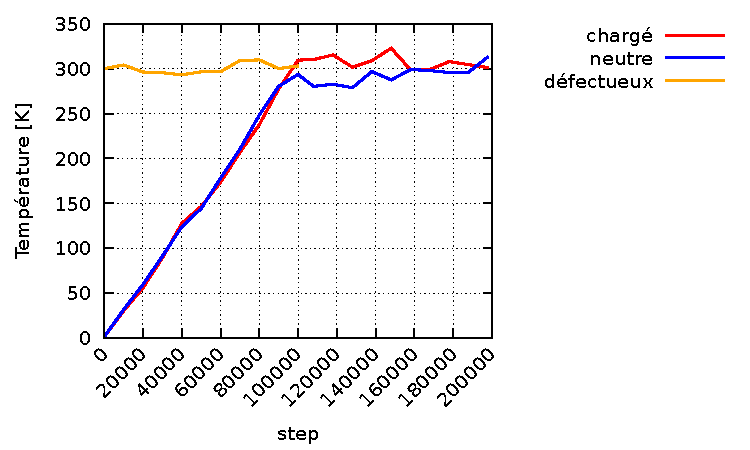
\includegraphics[width = \textwidth]{relaxation_temp.pdf}
        \caption{Température}
    \end{subfigure}%
    ~
    \begin{subfigure}[t]{.49 \textwidth}
        \centering
        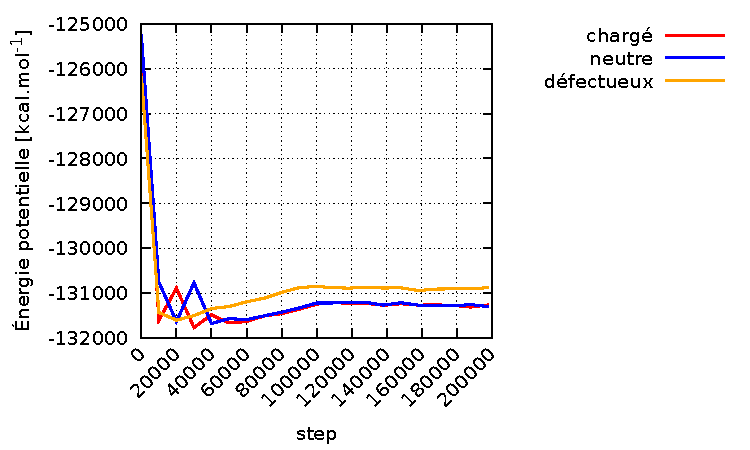
\includegraphics[width = \textwidth]{relaxation_epot.pdf}
        \caption{Énergie potentielle par atome}
    \end{subfigure}
    \begin{subfigure}[t]{.49 \textwidth}
        \centering
        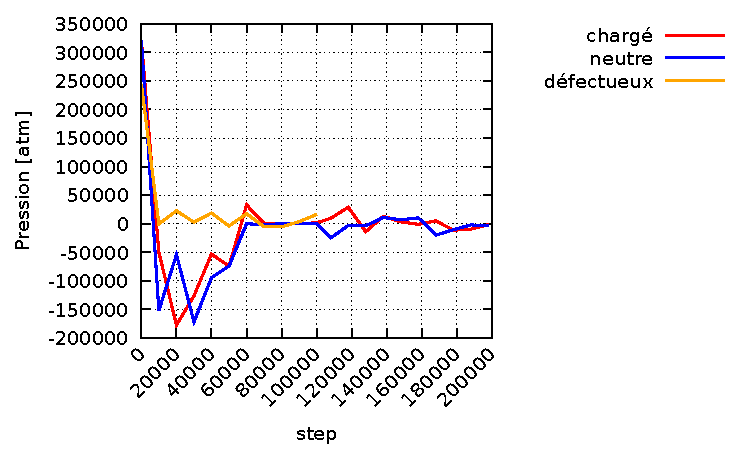
\includegraphics[width = \textwidth]{relaxation_press.pdf}
        \caption{Pression}
    \end{subfigure}
    \caption{Grandeurs thermodynamiques au cours de la relaxation et stabilisation}
    \label{fig:relaxation_thermo}
\end{figure}

\begin{figure}[h!]
    \centering
    \begin{subfigure}[t]{.49 \textwidth}
        \centering
        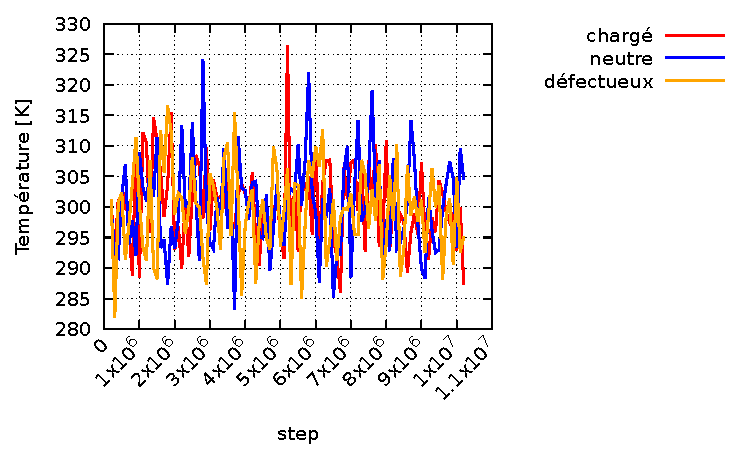
\includegraphics[width = \textwidth]{main_temp.pdf}
        \caption{Température}
    \end{subfigure}%
    ~
    \begin{subfigure}[t]{.49 \textwidth}
        \centering
        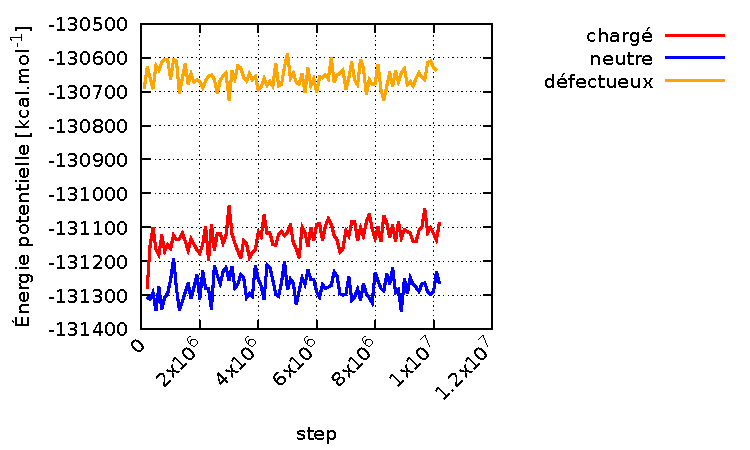
\includegraphics[width = \textwidth]{main_epot.pdf}
        \caption{Énergie potentielle par atome}
    \end{subfigure}
    \begin{subfigure}[t]{.49 \textwidth}
        \centering
        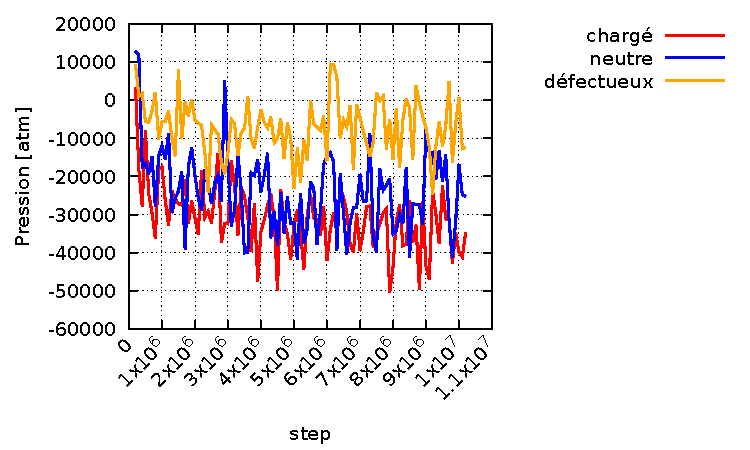
\includegraphics[width = \textwidth]{main_press.pdf}
        \caption{Pression}
    \end{subfigure}
    \caption{Grandeurs thermodynamiques au cours de la simulation principale}
    \label{fig:main_thermo}
\end{figure}

% Charge distribution on the electrode
    \subsubsection{Distribution des charges sur les électrodes}

La distribution des charges sur les électrodes est mesurée par la moyenne des charges au sein de certains groupes d'atomes. Ceux-ci sont : les atomes de carbone composant les couches extérieures des électrodes, les atomes des couches intérieures, les atomes voisins du défaut.\\
La \autoref{fig:charges_groupes} présente les différents graphes obtenus pour cette mesure pour les différents systèmes, les \autoref{fig:comparaison_ch-sc-defected} et \ref{fig:comparaison_ch-sc-neutral} présentent des comparaisons entre les systèmes, et le \autoref{tab:comparaison_charges} résume les moyennes des charges suivant le groupe d'atomes de carbone.

\begin{figure}[h!]
    \centering
    \begin{subfigure}[t]{.49 \textwidth}
        \centering
        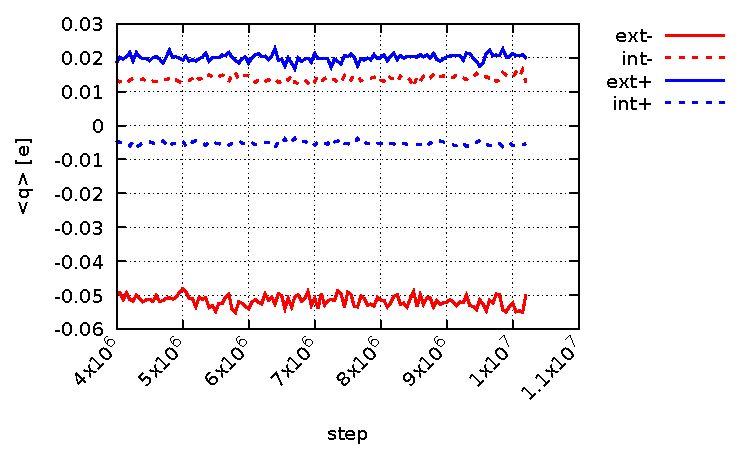
\includegraphics[width = \textwidth]{ch-sc_q-1.pdf}
        \caption{Pour le système chargé}
        \label{fig:charges_groupes_ch-sc}
    \end{subfigure}%
    ~
    \begin{subfigure}[t]{.49 \textwidth}
        \centering
        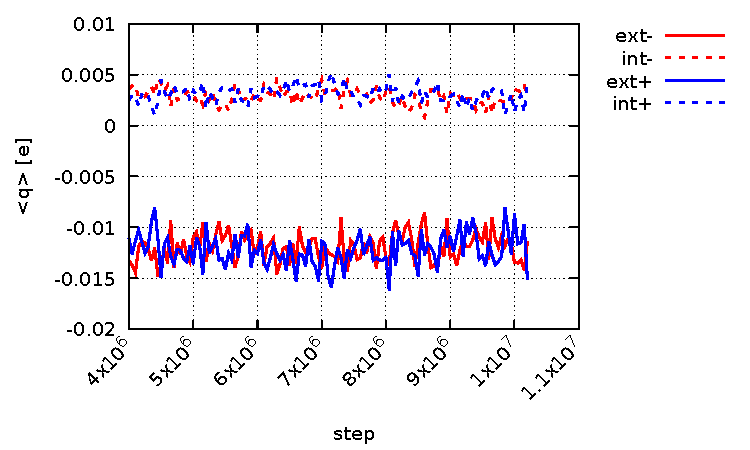
\includegraphics[width = \textwidth]{neutral_q-1.pdf}
        \caption{Pour le système non chargé}
        \label{fig:charges_groupes_neutral}
    \end{subfigure}
    
    \begin{subfigure}[t]{.49 \textwidth}
        \centering
        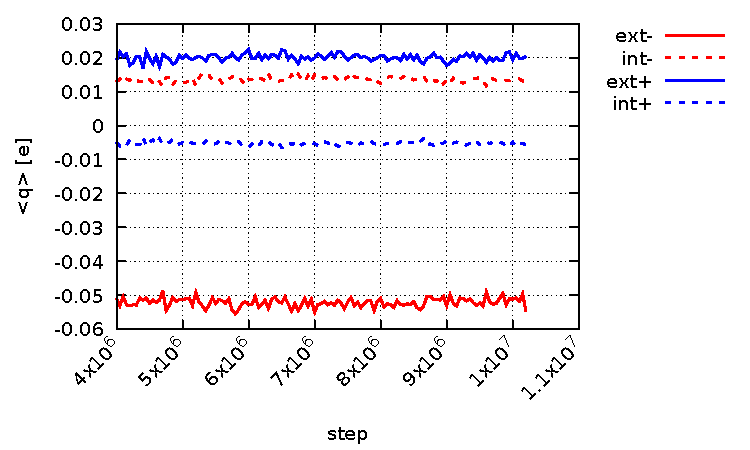
\includegraphics[width = \textwidth]{defected_q-1.pdf}
        \caption{Pour le système défectueux}
        \label{fig:charges_groupes_defected}
    \end{subfigure}

    \caption{Distribution des charges par groupes d'atomes. Les groupes d'atomes communs sont les carbones des couches intérieures et extérieures des deux électrodes ; Et pour le système défectueux il y a les atomes voisins du défaut}
    \label{fig:charges_groupes}
\end{figure}

\begin{figure}[h!]
    \centering
    \begin{subfigure}[t]{.49 \textwidth}
        \centering
        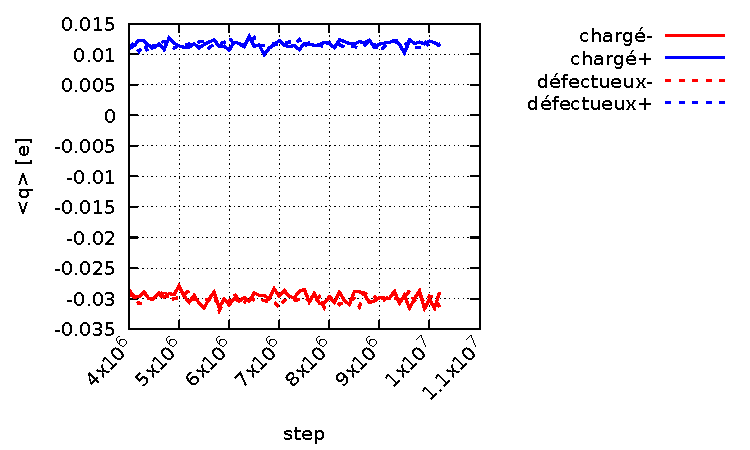
\includegraphics[width = \textwidth]{q_ch-sc-defected.pdf}
        \caption{Pour toutes les couches}
    \end{subfigure}%
    ~
    \begin{subfigure}[t]{.49 \textwidth}
        \centering
        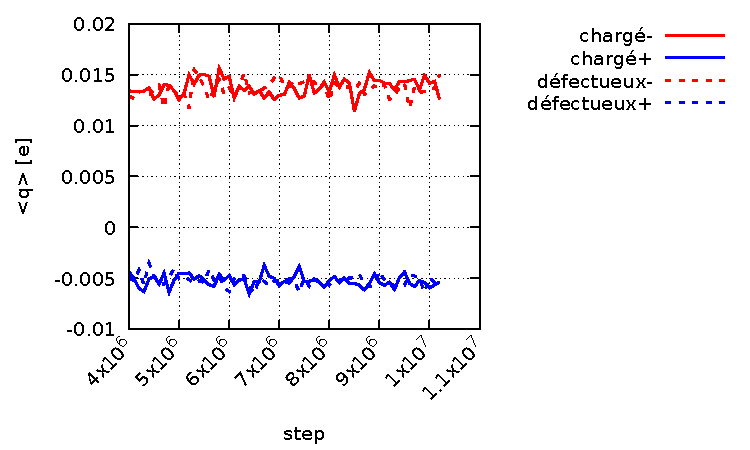
\includegraphics[width = \textwidth]{q_ch-sc-defected-inn.pdf}
        \caption{Pour les couches intérieures}
    \end{subfigure}

    \begin{subfigure}[t]{.49 \textwidth}
        \centering
        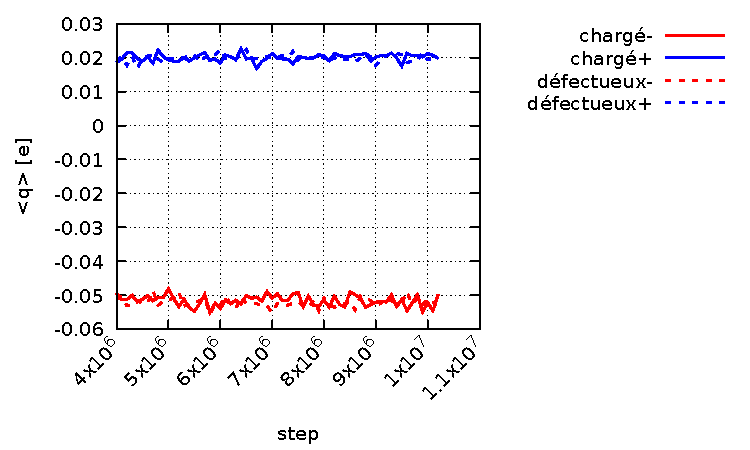
\includegraphics[width = \textwidth]{q_ch-sc-defected-out.pdf}
        \caption{Pour les couches extérieures}
    \end{subfigure}
    \caption{Comparaison des charges entre le système chargé et le système défectueux}
    \label{fig:comparaison_ch-sc-defected}
\end{figure}

\begin{figure}[h!]
    \centering
    \begin{subfigure}[t]{.49 \textwidth}
        \centering
        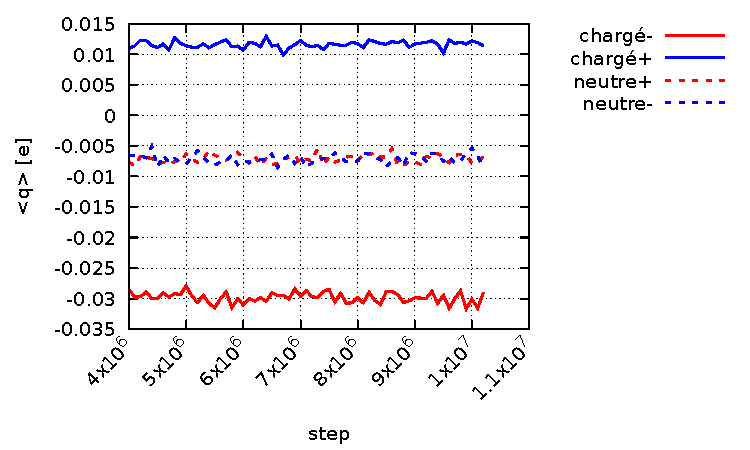
\includegraphics[width = \textwidth]{q_ch-sc-neutral.pdf}
        \caption{Pour toutes les couches}
    \end{subfigure}%
    ~
    \begin{subfigure}[t]{.49 \textwidth}
        \centering
        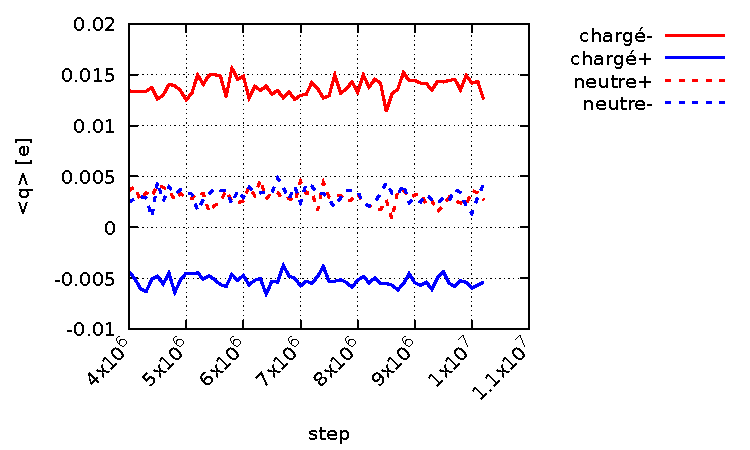
\includegraphics[width = \textwidth]{q_ch-sc-neutral-inn.pdf}
        \caption{Pour les couches intérieures}
    \end{subfigure}

    \begin{subfigure}[t]{.49 \textwidth}
        \centering
        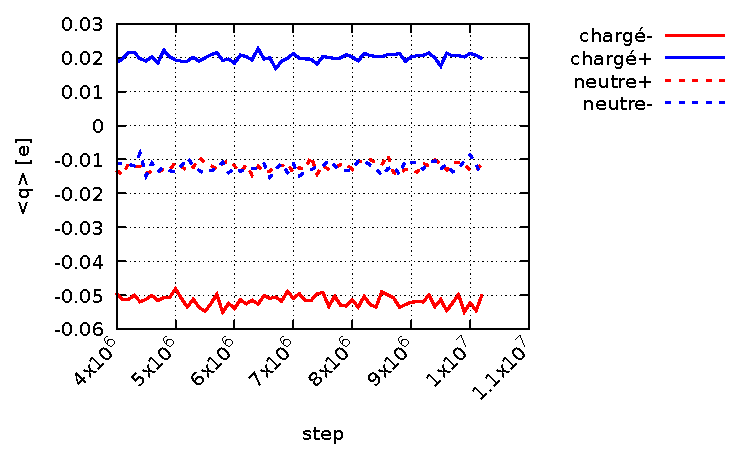
\includegraphics[width = \textwidth]{q_ch-sc-neutral-out.pdf}
        \caption{Pour les couches extérieures}
    \end{subfigure}
    \caption{Comparaison des charges entre le système chargé et le système non chargé}
    \label{fig:comparaison_ch-sc-neutral}
\end{figure}

\begin{table}[h!]
    \centering
    \begin{tabular}{c | c | c || c}
        \hline
        Système &Électrode &Couches &Moyenne des charges [\unit{\e}]\\
        \hline
        chargé &négative &toutes &\num{-0.0299}\\
         & &intérieures &\num{0.0138}\\
         & &extérieures &\num{-0.0517}\\
         &positive &toutes &\num{0.0116}\\
         & &intérieures &\num{-0.0052}\\
         & &extérieures &\num{0.0200}\\
        \hline
        neutre &négative &toutes &\num{-0.0070}\\
         & &intérieures &\num{0.0031}\\
         & &extérieures &\num{-0.0121}\\
        &positive &toutes &\num{-0.0071}\\
         & &intérieures &\num{0.0028}\\
         & &extérieures &\num{-0.0119}\\ 
        \hline
        défectueux &négative &toutes &\num{-0.0300}\\
         & &intérieures &\num{0.0135}\\
         & &extérieures &\num{-0.0519}\\
         &positive &toutes &\num{0.0116}\\
         & &intérieures &\num{-0.0052}\\
         & &extérieures &\num{0.0200}\\
        \hline
    \end{tabular}
    \caption{Tableau récapitulatif des moyennes des charges en fonction du groupe de carbone}
    \label{tab:comparaison_charges}
\end{table}

\clearpage

\textbf{Observations}\\
Pour les systèmes chargés (\autoref{fig:charges_groupes_ch-sc} et \ref{fig:charges_groupes_defected}, et \autoref{tab:comparaison_charges}), il semble que les charges des électrodes soient situées plutôt sur leurs couches extérieures : pour l'électrode négative les couches extérieures sont chargées négativement, tandis que pour l'électrode positive elles sont chargées positivement.

Pour le système neutre (\autoref{fig:charges_groupes_neutral}, et \autoref{tab:comparaison_charges}), nous pouvons voir un décalage de charges entre les couches : les couches extérieures sont chargées négativement tandis que les couches intérieures sont chargées positivement, de plus les couches extérieures sont plus chargées que les couches intérieures. Mais malgré ces décalages, les moyennes des charges sont quasimment les mêmes pour les deux électrodes et leurs couches respectives.

En comparant les systèmes chargés (\autoref{fig:comparaison_ch-sc-defected}, et \autoref{tab:comparaison_charges}), nous voyons que les charges des deux systèmes sont quasimment les mêmes pour les deux électrodes et leurs couches séparément.

En comparant les systèmes chargés au système non chargé (\autoref{fig:comparaison_ch-sc-neutral}, et \autoref{tab:comparaison_charges}), nous pouvons voir que pour les charges des électrodes des systèmes chargés sont presque à écarts égaux des charges du système non chargé. Cependant, l'écart de charges entre les couches intérieures et extérieures est plus grand pour l'électrode négative que pour l'électrode positive (\qtyrange[range-units = single]{125}{135}{\percent}).

\textbf{Interprétations}\\
La différence de charges entre les couches extérieures et intérieures peut avoir trois raisons :
\begin{itemize}
    \item La polarisation du système a pour conséquence d'attirer les charges d'une électrode vers l'autre ; Puisque le système est périodique selon la direction orthogonale aux surfaces des électrodes (selon la direction $[Oz)$), les charges d'une électrode sont attirées vers l'électrode opposée et son image périodique, c'est-à-dire vers les couches extérieures
    \item Au commencement de l'analyse des données (à partir de \qty{0.4}{\nano \second}), la double couche électrochimique (\edl{}) est déjà formée et les charges de chaque électrode sont concentrées à leurs interfaces avec l'électrolyte
    \item Les environnements des atomes de carbones influencent leurs propriétés (notamment leur charge) ; De plus, dans une approximation métallique les charges tendent à se diffuser vers la surface du métal
\end{itemize}

Quant au décalage de charges entre les couches du système non chargé, puisqu'il n'existe pas de différence de potentiel entre les électrodes il est possible que ce phénomène ne soit qu'une conséquence de l'interface entre l'électrode et l'électrolyte.

L'absence de différences notables entre les charges des systèmes chargés nous laisse penser que la présence du défaut n'influence pas la charge du système dans sa globalité.

Pour les écarts de charges entre les couches intérieures et extérieures du système chargé par rapport aux valeurs du système neutre, il n'y a pas de raison apparente. Cependant, le fait que pour les trois groupes d'atomes (couches intérieures, extérieures, et intégralité de l'électrode) il y ait un rapport d'environ $\num{1.25}\sim \num{1.35}$ nous laisse penser qu'il existe une raison sous-jacente et non évidente.

\clearpage
% Ions adsorption/displacement
    \subsubsection{Adsorption et déplacements des ions}

L'adsorption des ions est mesurée par deux grandeurs : la densité numérique d'ions dans l'électrolyte, et la fonction de ditribution radiale entre les ions et les carbones des électrodes.

Les \autoref{fig:densite} et \ref{fig:comparaison_densite} présentent la densité numérique d'ions dans l'électrolyte en fonction de la direction $[Oz)$ (correspondant à la direction orthogonale aux surfaces des électrodes) au début de l'analyse (à \qty{0.4}{\nano \second}) et à la fin (à \qty{1.0}{\nano \second}) pour les systèmes chargés et le système neutre.\\
Les \autoref{fig:rdf_ch-sc-neutral} et \ref{fig:rdf_ch-sc-defected}, elles montrent les \rdf{}s des ions sodium et hydroxyde de l'électrolyte par rapport aux carbones des couches extérieures des deux électrodes des trois systèmes. Et la \autoref{fig:rdf_sp} compare la \rdf{} des ions sodium et des carbones voisins du défaut du système défectueux à d'autres carbones.

\begin{figure}[h!]
    \centering
    \begin{subfigure}[t]{.49 \textwidth}
        \centering
        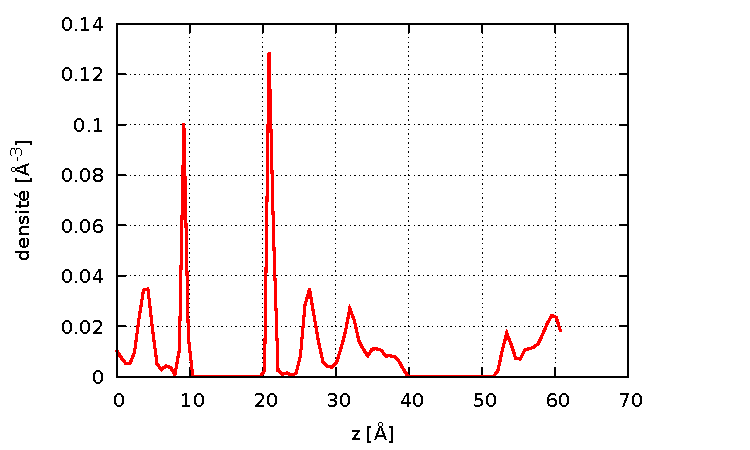
\includegraphics[width = \textwidth]{ch-sc_average_density.pdf}
        \caption{Pour le système chargé}
    \end{subfigure}%
    ~
    \begin{subfigure}[t]{.49 \textwidth}
        \centering
        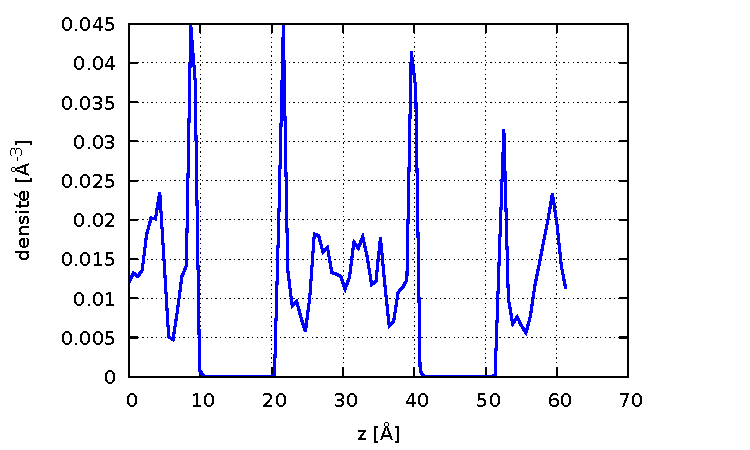
\includegraphics[width = \textwidth]{neutral_average_density.pdf}
        \caption{Pour le système non chargé}
    \end{subfigure}

    \begin{subfigure}[t]{.49 \textwidth}
        \centering
        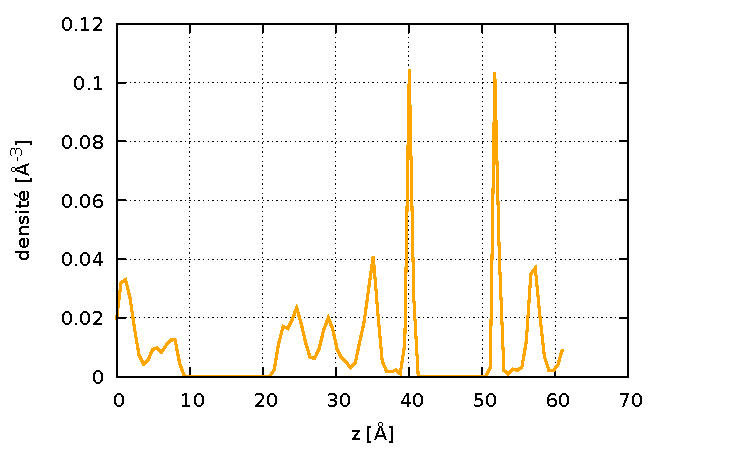
\includegraphics[width = \textwidth]{defected_average_density.pdf}
        \caption{Pour le système défectueux}
    \end{subfigure}
    \caption{Densités numériques moyennes d'ions sodium dans l'électrolyte}
    \label{fig:densite}
\end{figure}

\begin{figure}[h!]
    \centering
    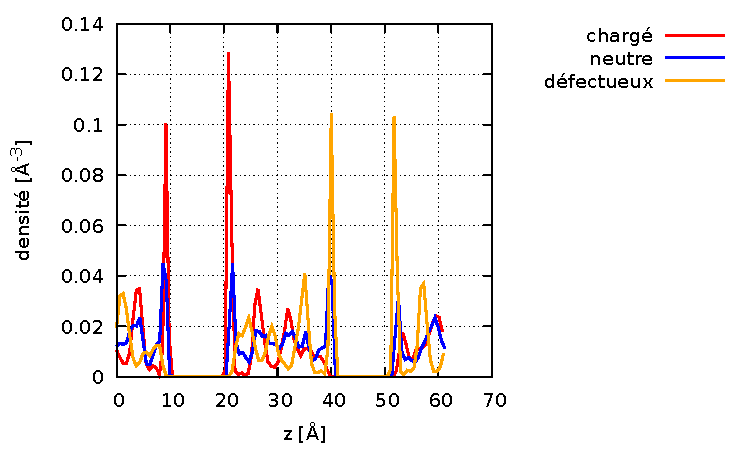
\includegraphics[width = \textwidth]{densities.pdf}
    \caption{Comparaisons des densités numériques moyennes. Le système défectueux a ses électrodes échangées (la positive à la place de la négative) par rapport au système chargé.}
    \label{fig:comparaison_densite}
\end{figure}

\begin{figure}[h!]
    \centering
    \begin{subfigure}[t]{.49 \textwidth}
        \centering
        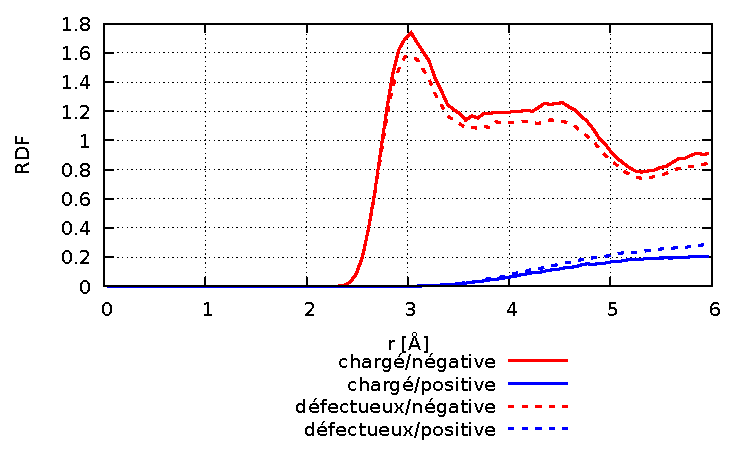
\includegraphics[width = \textwidth]{rdf_ch-sc-defected-Na.pdf}
        \caption{Pour les ions sodium}
    \end{subfigure}%
    ~
    \begin{subfigure}[t]{.49 \textwidth}
        \centering
        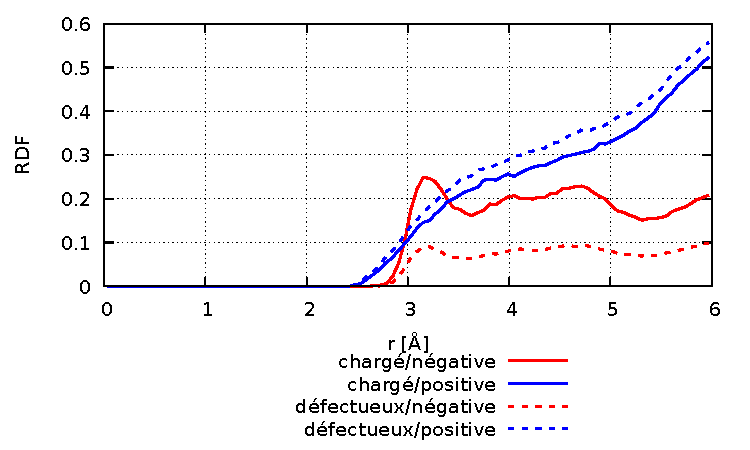
\includegraphics[width = \textwidth]{rdf_ch-sc-defected-OH.pdf}
        \caption{Pour les ions hydroxyde}
    \end{subfigure}

    \begin{subfigure}[t]{.49 \textwidth}
        \centering
        \includegraphics[width = \textwidth]{rdf_ch-sc-defected-NaOH.pdf}
        \caption{Pour tous les ions, par rapport à leurs électrodes respectives}
    \end{subfigure}
    \caption{Comparaison des \rdf{}s des ions par rapport aux carbones des électrodes entre le système chargé et le système défectueux}
    \label{fig:rdf_ch-sc-defected}
\end{figure}

\begin{figure}[h!]
    \centering
    \begin{subfigure}[t]{.49 \textwidth}
        \centering
        \includegraphics[width = \textwidth]{rdf_ch-sc-neutral-Na.pdf}
        \caption{Pour les ions sodium}
    \end{subfigure}%
    ~
    \begin{subfigure}[t]{.49 \textwidth}
        \centering
        \includegraphics[width = \textwidth]{rdf_ch-sc-neutral-OH.pdf}
        \caption{Pour les ions hydroxyde}
    \end{subfigure}

    \begin{subfigure}[t]{.49 \textwidth}
        \centering
        \includegraphics[width = \textwidth]{rdf_ch-sc-neutral-NaOH.pdf}
        \caption{Pour les tous ions, par rapport à leurs électrodes respectives}
    \end{subfigure}
    \caption{Comparaison des \rdf{}s des ions par rapport aux carbones des électrodes entre le système chargé et le système neutre}
    \label{fig:rdf_ch-sc-neutral}
\end{figure}

\begin{figure}[h!]
    \centering
    \begin{subfigure}[t]{.49 \textwidth}
        \centering
        \includegraphics[width = \textwidth]{rdf_ch-sc-defected-sp.pdf}
        \caption{Avec les carbones de l'électrode négative du système chargé}
    \end{subfigure}%
    ~
    \begin{subfigure}[t]{.49 \textwidth}
        \centering
        \includegraphics[width = \textwidth]{rdf_defected.pdf}
        \caption{Avec les carbones de l'électrode négative du système défectueux}
    \end{subfigure}
    \caption{Comparaison de la \rdf{} des ions sodium et des voisins du défaut}
    \label{fig:rdf_sp}
\end{figure}

\clearpage
\textbf{Observations}\\
Pour les densités numériques moyennes des ions sodium selon l'axe $[Oz)$ (\autoref{fig:densite}), nous pouvons dire que pour les systèmes chargés les ions sodium se regroupent près l'électrode négative (avec des pics de densité jusqu'à \num{4} fois plus grands qu'ailleurs dans l'électrolyte) ; Et pour le système neutre nous voyons des pics de densité moins important près des deux électrodes (environ \num{2} fois la valeur de la densité ailleurs dans l'électrolyte).

En observant attentivement, nous pouvons décerner un pattern pour les trois courbes : un pic intense près d'une des électrodes, puis une baisse de densité suivie de plusieurs pics à moyenne voire basse intensité.

En comparant les densités numériques des systèmes (\autoref{fig:comparaison_densite}), il est clair que les pics près des électrodes sont \num{2} à \num{3} fois plus intenses pour les systèmes chargés que pour le système non chargé.

En examinant les \rdf{}s, nous pouvons observer que :
\begin{itemize}
    \item la \rdf{} d'un ion est plus élevée et structurée lorsque prise par rapport aux carbones de l'électrode qui l'attire
    \item les \rdf{}s des systèmes chargés sont légèrement décalées mais dessinent les mêmes formes (\autoref{fig:rdf_ch-sc-defected})
    \item les \rdf{}s du système neutre sont plus uniformes que celles des systèmes chargés (\autoref{fig:rdf_ch-sc-neutral})
    \item pour tous les systèmes, les \rdf{}s des ions sodium sont globalement plus élevées et possèdent des pics plus prononcés que les \rdf{}s des ions hydroxyde
    \item la \rdf{} du sodium par rapport aux voisins du défaut est très similaire aux \rdf{}s par rapport aux autres carbones (\autoref{fig:rdf_sp})
\end{itemize}

\textbf{Interprétations}\\
Les différences de densités numériques entre les systèmes chargés et le système neutre semblent intuitives : les ions sodium sont plus dispersés pour le système neutre que pour le système chargé, à cause de l'application de la différene de potentiel, et les pics de densité près de l'électrode négative sont plus importants pour les sytèmes chargés à cause de la différence de potentiel appliquée.

Puisque les densités numériques des trois systèmes montrent un même pattern, il est très probable que ce ne soit pas un hasard : nous pouvons penser qu'une couche d'ions est fortement attirée par l'électrode, et le reste des ions en excès reste dans une couche plus éloignée, dite de \emph{diffusion}.

À cause de leur charge négative, même en l'absence de polarisation (\autoref{tab:comparaison_charges}), les deux électrodes du système neutre attirent les ions sodium de l'électrolyte.

Les \rdf{}s nous permettent d'étayer ces réflexions :
\begin{itemize}
    \item puisque les ions sont attirés par leur électrode opposée, la \rdf{} correspondante sera plus intense. Avec le pattern de densité décrit précédemment, il est également normal d'observer des pics pour les \rdf{}s
    \item à l'inverse pour le système non chargé, les \rdf{}s seront plus uniformes et moins intenses
\end{itemize}

Malgré cela, la différence des \rdf{}s des ions hydroxyde par rapport aux ions sodium n'est pas simple à interpréter : elle peut venir d'un problème d'implémentation ou d'un phénomène physique.\\
En effet, puisque le potentiel que nous utilisons est réactif, les atomes n'appartiennent pas à des molécules prédéfinies et ils peuvent alors se lier et se séparer les uns des autres. Cela rend alors le travail de sélection des ions plus difficile. Pour cette étude, nous avons choisi de faire simplement : à chaque image de la trajectoire de simulation, nous avons sélectionné tous les atomes d'oxygène et d'hydrogène, calculé les liaisons pouvant exister entre eux, et sélectionné seulement les atomes d'oxygène possédant moins de deux liaisons. Malgré qu'une bonne partie devrait être de \emph{vrais} ions hydroxyde, les atomes sélectionnés sont plus nombreux que le nombre initial d'ions de l'électrolyte pouvant ainsi causer des erreurs de calculs.\\
S'il n'y avait pas d'erreur, alors il est probable que cette différence soit causée par les réactions entre les ions hydroxyde et les molécules d'eau, perturbant la distribution des ions autour des électrodes.\\
Dans tous les cas, nous ne pouvons pas affirmer si les \rdf{}s des ions hydroxydes sont différentes de celles des ions sodium à cause de la charge différente des électrode (\autoref{tab:comparaison_charges}) ou à cause de la nature des ions.

Enfin, la comparaison des \rdf{}s du sodium par rapport aux voisins du défaut et des carbones des électrodes négatives des systèmes chargés ne montre pas de grande différence. Cela pourrait vouloir dire qu'un tel défaut ou un défaut seul ne permette pas de voir une grande différence ; Cette différence pourrait surgir avec un système de plus grande taille, ou pour des simulations plus longues avec de plus grandes statistiques.

% Discussion of the study
    \subsection{Discussion}

Les résultats obtenus pourraient être améliorés pour une prochaine étude en :
\begin{itemize}
    \item équilibrant la simulation principale \emph{avant} d'appliquer la différence de potentiel afin de pouvoir observer sur un même système la formation de l'\edl{}, les variations de charges des électrodes (lorsque le voltage se met en place), et pouvoir calculer deux densités numériques moyennes d'ions différentes [avant et après la mise en place de la différence de potentiel]
    \item augmentant la taille du système, de manière à obtenir plus de statistiques
    \item complexifiant progressivement le système, par exemple en créant un pore artificiel dans l'électrode, ou encore en créant un tunnel dans l'électrode pour simuler un réseau de pore, dans le but de voir l'influence d'une telle modification sur le système
    \item remplaçant les ions hydroxydes initiaux par d'autres anions, comme par exemple les ions chlore, afin de les tracer plus facilement dans l'électrolyte et de déterminer si les différences que nous avons observé provenaient de la nature des ions utilisés ou du système lui-même
\end{itemize}

\clearpage


% Conclusion
\section{Conclusion}

    
Pour cette étude, nous avons fait le choix de prendre un système modèle simple, afin de comprendre les fondements des mécanismes animant les électrodes capacitives. Nous avons voulu étudier la distribution des charges au sein des électrodes et l'adsorption des ions à la surface des électrodes, pour un tel système.

Ce travail nous a apporté certaines réponses :
\begin{itemize}
    \item La distribution des charges au sein des électrodes capacitives n'est jamais uniforme, même lorsqu'aucune polarisation n'est mise en place
    \item Les charges d'une électrode capacitive ont tendance à se placer sur ses couches extérieures, et les couches intérieures sont même de charge opposée
    \item Une structure est en place dans l'électrolyte, et celle-ci est amplifiée lorsque l'on applique une différence de potentiel entre les électrodes
\end{itemize}
ainsi que de nouvelles questions :
\begin{itemize}
    \item D'où proviennent les différences entre le comportement des ions sodium et hydroxyde ?
    \item Est-ce que la présence d'un défaut structurel impacte le système de manière significative ?
    \item Dans quelle mesure le système se retrouve fortement impacté par les défauts qu'il possède ?
\end{itemize}

Et il mérite d'être poursuivi, car il reste encore des pistes à explorer, comme le remplacement des anions, l'agrandissement du système, l'ajout de défaut de types différents (ajout d'atome sur la surface, ajout d'un pore tout entier voire d'une cavité dans l'électrode), ou encore l'ajout de défauts supplémentaires.


\clearpage


% Annexes
\appendix
\pagenumbering{roman}
\section{Construction des configurations initiales avec \packmol{}} \label{apdx:packmol}

    
Nous préparons les systèmes avec un outil libre nommé \packmol{}. Il permet de dupliquer, d'ajouter et d'agencer des molécules pour des sytèmes relativement complexes. Pour un système composé uniquement de molécules d'eau des solutions \qty{100}{\percent} \lammps{} existent mais il est beaucoup plus simple et rapide d'utiliser \packmol{}.

Pour montrer notre utilisation de cet outil, nous présentons un exemple pour la préparation d'un système composé uniquement de molécules d'eau.

Soit une boîte de simulation cubique de côté : $X = Y = Z = \qty{20.0}{\angstrom}$. En prenant $\rho_{\ce{H2O}} = $\qty{1000}{\kilo \gram \per \cubic \meter}, $V = \qty{8.0e-27}{\cubic \meter}$, $\mathcal{N}_A = $\qty{6.022e+23}{\per \mole}, et $M_{\ce{H2O}} = $\qty{1.801e-02}{\kilo \gram \per \mole}, nous trouvons le nombre de molécules d'eau à répartir dans la boîte de simulation : $N \approx \num{267}$.

Pour des molécules d'eau, nous prendrons une tolérance de $\mathtt{tol} = \qty{2.5}{\angstrom}$ pour s'assurer que les molécules d'eau ne se chevauchent pas. Et pour anticiper l'application des conditions aux limites périodiques, nous réduisons la région où répartir les molécules à : $X^m = Y^m = Z^m = \qty{1.25}{\angstrom}$ et $X^M = Y^M = Z^M = \qty{18.75}{\angstrom}$, pour qu'elles ne se chevauchent pas même à travers les conditions aux limites périodiques.

Une fois toutes ces informations calculées nous pouvons écrire le script qui sera donné à \packmol{} :
\begin{lstlisting}[caption={Répartition des molécules d'eau}, label={lst:packmol_example}]
tolerance 2.5
output output.xyz
filetype xyz
structure water.xyz
    number 267
    inside box 1.25 1.25 1.25 18.75 18.75 18.75
end structure
\end{lstlisting}
où \lstinline!water.xyz! est un fichier comprenant les positions des atomes composant une molécule d'eau.

\clearpage

\section{Conversion des fichiers de configurations initiales au format \lammps{}} \label{apdx:conversion_lammps}

        \subsection{Détermination des listes de molécules et de liaisons}

Pour effectuer des simulations de systèmes tels que le précédent, il est nécessaire de fournir un fichier de données à LAMMPS. Celui-ci doit se présenter sous un format spécifique et contenir les informations du système (\href{https://docs.lammps.org/read_data.html#format-of-a-data-file}{manuel utilisateur de LAMMPS}).

Il est donc nécessaire de pré-traiter les données fournies par le fichier XYZ produit par PACKMOL pour les formater et les soumettre à LAMMPS.

	\subsubsection{Format du fichier de données LAMMPS}

\textbf{En-tête du fichier}\\
L'en-tête du fichier de notre simulation doit comprendre les champs suivants :
\begin{itemize}
	\item \lstinline!atoms!, le nombre d'atomes
	\item \lstinline!bonds!, le nombre de liaisons
	\item \lstinline!angles!, le nombre d'angles
	\item \lstinline!atom types!, le nombre de types d'atomes
	\item \lstinline!bond types!, le nombre de types de liaisons
	\item \lstinline!angle types!, le nombre de types d'angles
	\item \lstinline!xlo xhi!, les limites de la boîte selon l'axe $[Ox)$
	\item \lstinline!ylo yhi!, les limites de la boîte selon l'axe $[Oy)$
	\item \lstinline!zlo zhi!, les limites de la boîte selon l'axe $[Oz)$
\end{itemize}
où chaque ligne doit se présenter sous la forme
\begin{lstlisting}
value(s)	keyword(s)
\end{lstlisting}

\textbf{Corps du fichier}\\
Le corps du fichier de notre simulation doit comprendre les sections suivantes :
\begin{itemize}
	\item \lstinline!Masses!, avec le format
\begin{lstlisting}
atom-type	mass
\end{lstlisting}
	\item \lstinline!Atoms!, avec le format \lstinline!full!
\begin{lstlisting}
atom-ID 	molecule-ID 	atom-type	q	x	y	z
\end{lstlisting}
	\item \lstinline!Angles!, avec le format
\begin{lstlisting}
angle-ID	angle-type	atom1	atom2	atom3
\end{lstlisting}
	\item \lstinline!Bonds!, avec le format
\begin{lstlisting}
bond-ID 	bond-type	atom1	atom2
\end{lstlisting}
\end{itemize}

	\subsubsection{Traitement des données}

Pour le traitement des données, il est important de se rendre compte que les données suivantes doivent être renseignées par l'utilisateur :
\begin{itemize}
	\item le nombre de types d'atomes
	\item le nombre de types de liaisons
	\item le nombre de types d'angles
	\item les limites de l'espace
	\item les correspondances types d'atomes-masses
	\item les correspondances types d'atomes-charges
\end{itemize}

Et les données restantes doivent être déterminées par un script :
\begin{itemize}
	\item le nombre d'atomes
	\item le nombre de liaisons
	\item le nombre d'angles
	\item les positions des atomes
	\item les atomes mis en jeu pour les liaisons
	\item les atomes mis en jeu pour les angles
\end{itemize}

Enfin, le diagramme de la \autoref{fig:donnees_flux} nous permet de dire qu'il faudra déterminer les données du corps du fichier avant de déterminer les données de l'en-tête.

\begin{figure}[h!]
	\centering
	\includegraphics[scale=1]{donnees-flux.pdf}
	\caption{Détermination des éléments du fichier de données}
	\label{fig:donnees_flux}
\end{figure}

\textbf{Détermination des liaisons}\\
Pour déterminer les liaisons entre les atomes du système nous nous basons sur les distances inter-atomiques. Ceci nous permet de concevoir le diagramme de la \autoref{fig:donnees_liaisons} et l'\autoref{alg:liaisons}.

\begin{figure}[h!]
	\centering
	\includegraphics[width=\linewidth]{donnees-liaisons.pdf}
	\caption{Détermination des liaisons}
	\label{fig:donnees_liaisons}
\end{figure}

\begin{algorithm}[h!]
	\Donnees{$\mathtt{N_{part}}$ le nombre de particules, $\mathtt{r}$ les positions des particules, $\mathtt{N_{tliaisons}}$ le nombre de types de liaisons, $\mathtt{t}$ les seuils des liaisons}
	\Sortie{$\mathtt{L}$ le tableau des indices des paires de particules liées}
	\Deb%
	{
		\Pour{\upshape \bfseries $\mathtt{i}$ de \num{0} à $\mathtt{N_{part}}$}%
		{
			\Pour{\upshape \bfseries $\mathtt{j}$ de $\mathtt{i + 1}$ à $\mathtt{N_{part}}$}%
			{
				$\mathtt{r_{ij} \gets |r_i - r_j|}$\;
				\Pour{\upshape \bfseries $\mathtt{k}$ de \num{0} à $\mathtt{N_{tliaisons}}$}%
				{
					\Si{$\mathtt{t_k} \leq \mathtt{r_{ij}} \leq \mathtt{t_{k + 1}}$}%
					{
						\texttt{ajouter}$\mathtt{(L_k, [i, j])}$\;
					}
				}
			}
		}
		\Retour{$\mathtt{L}$}
	}
	\caption{Détermination des liaisons}
	\label{alg:liaisons}
\end{algorithm}

\textbf{Détermination des molécules}\\
Pour déterminer les molécules, nous nous basons sur les liaisons en partant du principe qu'une molécule est un ensemble d'atomes liés entre eux au moins deux à deux.\\
Par exemple avec un tableau de liaisons $\mathtt{L = [[[1, 2], [2, 3]]]}$, on veut avoir le résultat $\mathtt{M = [[1, 2, 3]]}$ de sorte à ce que l'entrée $\mathtt{M_0}$ corresponde à la première molécule, mettant en jeu les atomes numérotés \num{1}, \num{2} et \num{3}.

Nous pouvons alors concevoir le diagramme de la \autoref{fig:donnees_molecules} et l'\autoref{alg:molecules}.

\begin{figure}[h!]
	\centering
	\includegraphics[width=\linewidth]{donnees-molecules.pdf}
	\caption{Détermination des molécules}
	\label{fig:donnees_molecules}
\end{figure}

\begin{algorithm}[h!]
	\Donnees{$\mathtt{L}$ le tableau des indices des paires de particules liées}
	\Sortie{$\mathtt{M}$ le tableau des indices des atomes appartenant aux mêmes molécules}
	\Deb%
	{
		$\mathtt{L' \gets concatener(L, axe=0)}$\;
		\Pour{\bfseries \upshape $\mathtt{i}$ de \num{0} à $\mathtt{nombre(L')}$}%
		{
			$\mathtt{ajoute \gets faux}$\;
			\PourCh{\bfseries \upshape $\mathtt{atome}$ de $\mathtt{L'_i}$}%
			{
				\PourCh{\bfseries \upshape $\mathtt{molecule}$ de $\mathtt{M}$}%
				{
					\Si{$\mathtt{atome \in molecule}$}%
					{
						$\mathtt{retirer(L'_i, atome)}$\;
						$\mathtt{ajouter(molecule, L'_i)}$\;
						$\mathtt{ajoute \gets vrai}$\;
						$\mathtt{stopper}$\;
					}
				}
				\Si{$\mathtt{ajoute}$}%
				{
					$\mathtt{stopper}$\;
				}
			}
			\Si{$\mathtt{non~ajoute}$}%
			{
				$\mathtt{ajouter(M, L'_i)}$\;
			}
		}
		\Retour{$\mathtt{M}$}
	}
	\caption{Détermination des molécules}
	\label{alg:molecules}
\end{algorithm}

\textbf{Détermination des angles}\\
Pour déterminer les angles nous nous basons sur les molécules. Nous pouvons concevoir le diagramme de la \autoref{fig:donnees_angles}, cependant une méthode alternative adaptée pour un système à un type d'angle fonctionne et a été implémentée directement.

\begin{figure}[h!]
	\centering
	\includegraphics[width=\linewidth]{donnees-angles.pdf}
	\caption{Détermination des angles}
	\label{fig:donnees_angles}
\end{figure}

\textbf{Implémentation}\\
Ces algorithmes ont pu être implémentés pour construire un script permettant, à partir d'un fichier d'entrée et du fichier de configuration au format XYZ, d'écrire un fichier de données LAMMPS automatiquement.

Le fichier d'entrée doit contenir les informations sur le système à simuler. Un exemple est présenté par le \autoref{lst:conversion_input}.

\begin{lstlisting}[caption={Fichier d'entrée pour la conversion}, label={lst:conversion_input}]
# input.txt
configuration_file: init.xyz
output_file: data.lammps
atom_types: O H
	masses: 15.9994 1.008
	charges: -0.8476 0.4238
bond_types: 1
	thresholds: 0.90 1.00
angle_types: 1
space_boundaries: 0.0 0.0 0.0 6.0 6.0 6.0
\end{lstlisting}

Et le résultat est présenté par un fichier tel que présenté par le \autoref{lst:conversion_sortie}.

\begin{lstlisting}[caption={Fichier de sortie de la conversion}, label={lst:conversion_sortie}]
# data.lammps
LAMMPS Description

  801 atoms
  534 bonds
  267 angles

Masses

1 15.9994 # O
2 1.008 # H
...

Atoms

1 1 2 0.4238 4.978146 3.160309 2.519717
2 1 1 -0.8476 5.220404 2.390845 1.990387
...

Bonds

1 1 1 2 
2 1 2 3 
...

Angles

1 1 1 2 3
2 1 4 5 6
...
\end{lstlisting}
\clearpage

\section{Traitement des données de simulation}

    
Le traitement des données a été fait avec des programme en C. Les modules de traitement de données sont disponibles sur \href{https://github.com/heiariilouchao/stage_M2.git}{Github}.
\clearpage

% References
\pagenumbering{gobble}
\printbibliography

\end{document}